% ===========================================================================
%  Figure block for "A Penalized Kernel Neural Network for Complex Genetic
%  Risk Prediction Analysis".  Paste into the manuscript; the PDFs sit beside
%  this file.
%
%  Preamble requirements:
%     \usepackage{graphicx}
%     (no \usepackage{rotating} needed: every figure is portrait)
%     \graphicspath{{plot/}}    % or adjust the paths below
%
%  Figures 2 and 3 are 9 rows (architecture) x 4 columns (SNP density) and are
%  taller than they are wide, so they are sized by HEIGHT: at 0.9\textheight
%  they come out about 5.8in wide and fit a portrait page.  They are still
%  dense -- 36 panels -- and read best at full size in supplementary material.
% ===========================================================================


% ---------------------------------------------------------------- Figure 1
% NOTE: this caption was written without being able to render the diagram
% (no PDF rasteriser on the cluster).  Check it against the figure.
\begin{figure}[htbp]
  \centering
  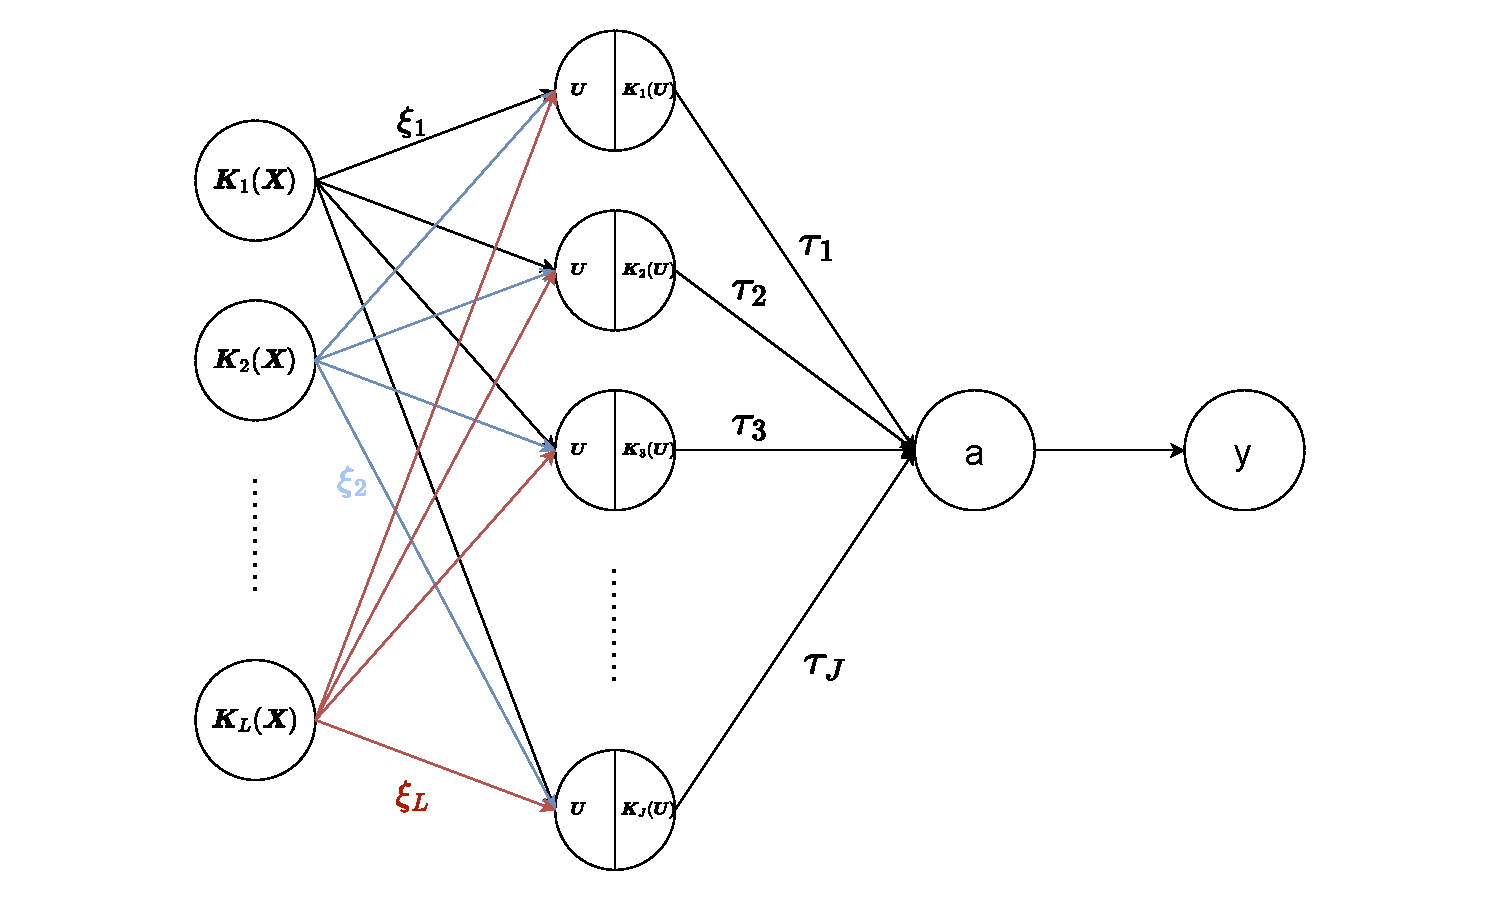
\includegraphics[width=\textwidth]{KNN_structure.pdf}
  \caption{Structure of the penalized kernel neural network (PKNN).  Genotypes
  are grouped into biologically defined regions, each region contributing one
  input kernel.  The hidden layer combines these kernels through random
  weights, so that the induced covariance of the network output is a linear
  combination of kernel products; the network is therefore equivalent to a
  linear mixed model whose variance components are the combination weights.
  With the interaction basis, ten regions generate 67 components: an identity
  term, ten main-effect kernels $K_i$, and the Hadamard products
  $K_i \circ K_j$, which reproduce exactly the kernel of the explicit pairwise
  cross-products between regions.  Estimation and selection of the variance
  components are carried out by penalized MINQUE.}
  \label{fig:knn-structure}
\end{figure}


% ---------------------------------------------------------------- Figure 2
\begin{figure}[p]
  \centering
  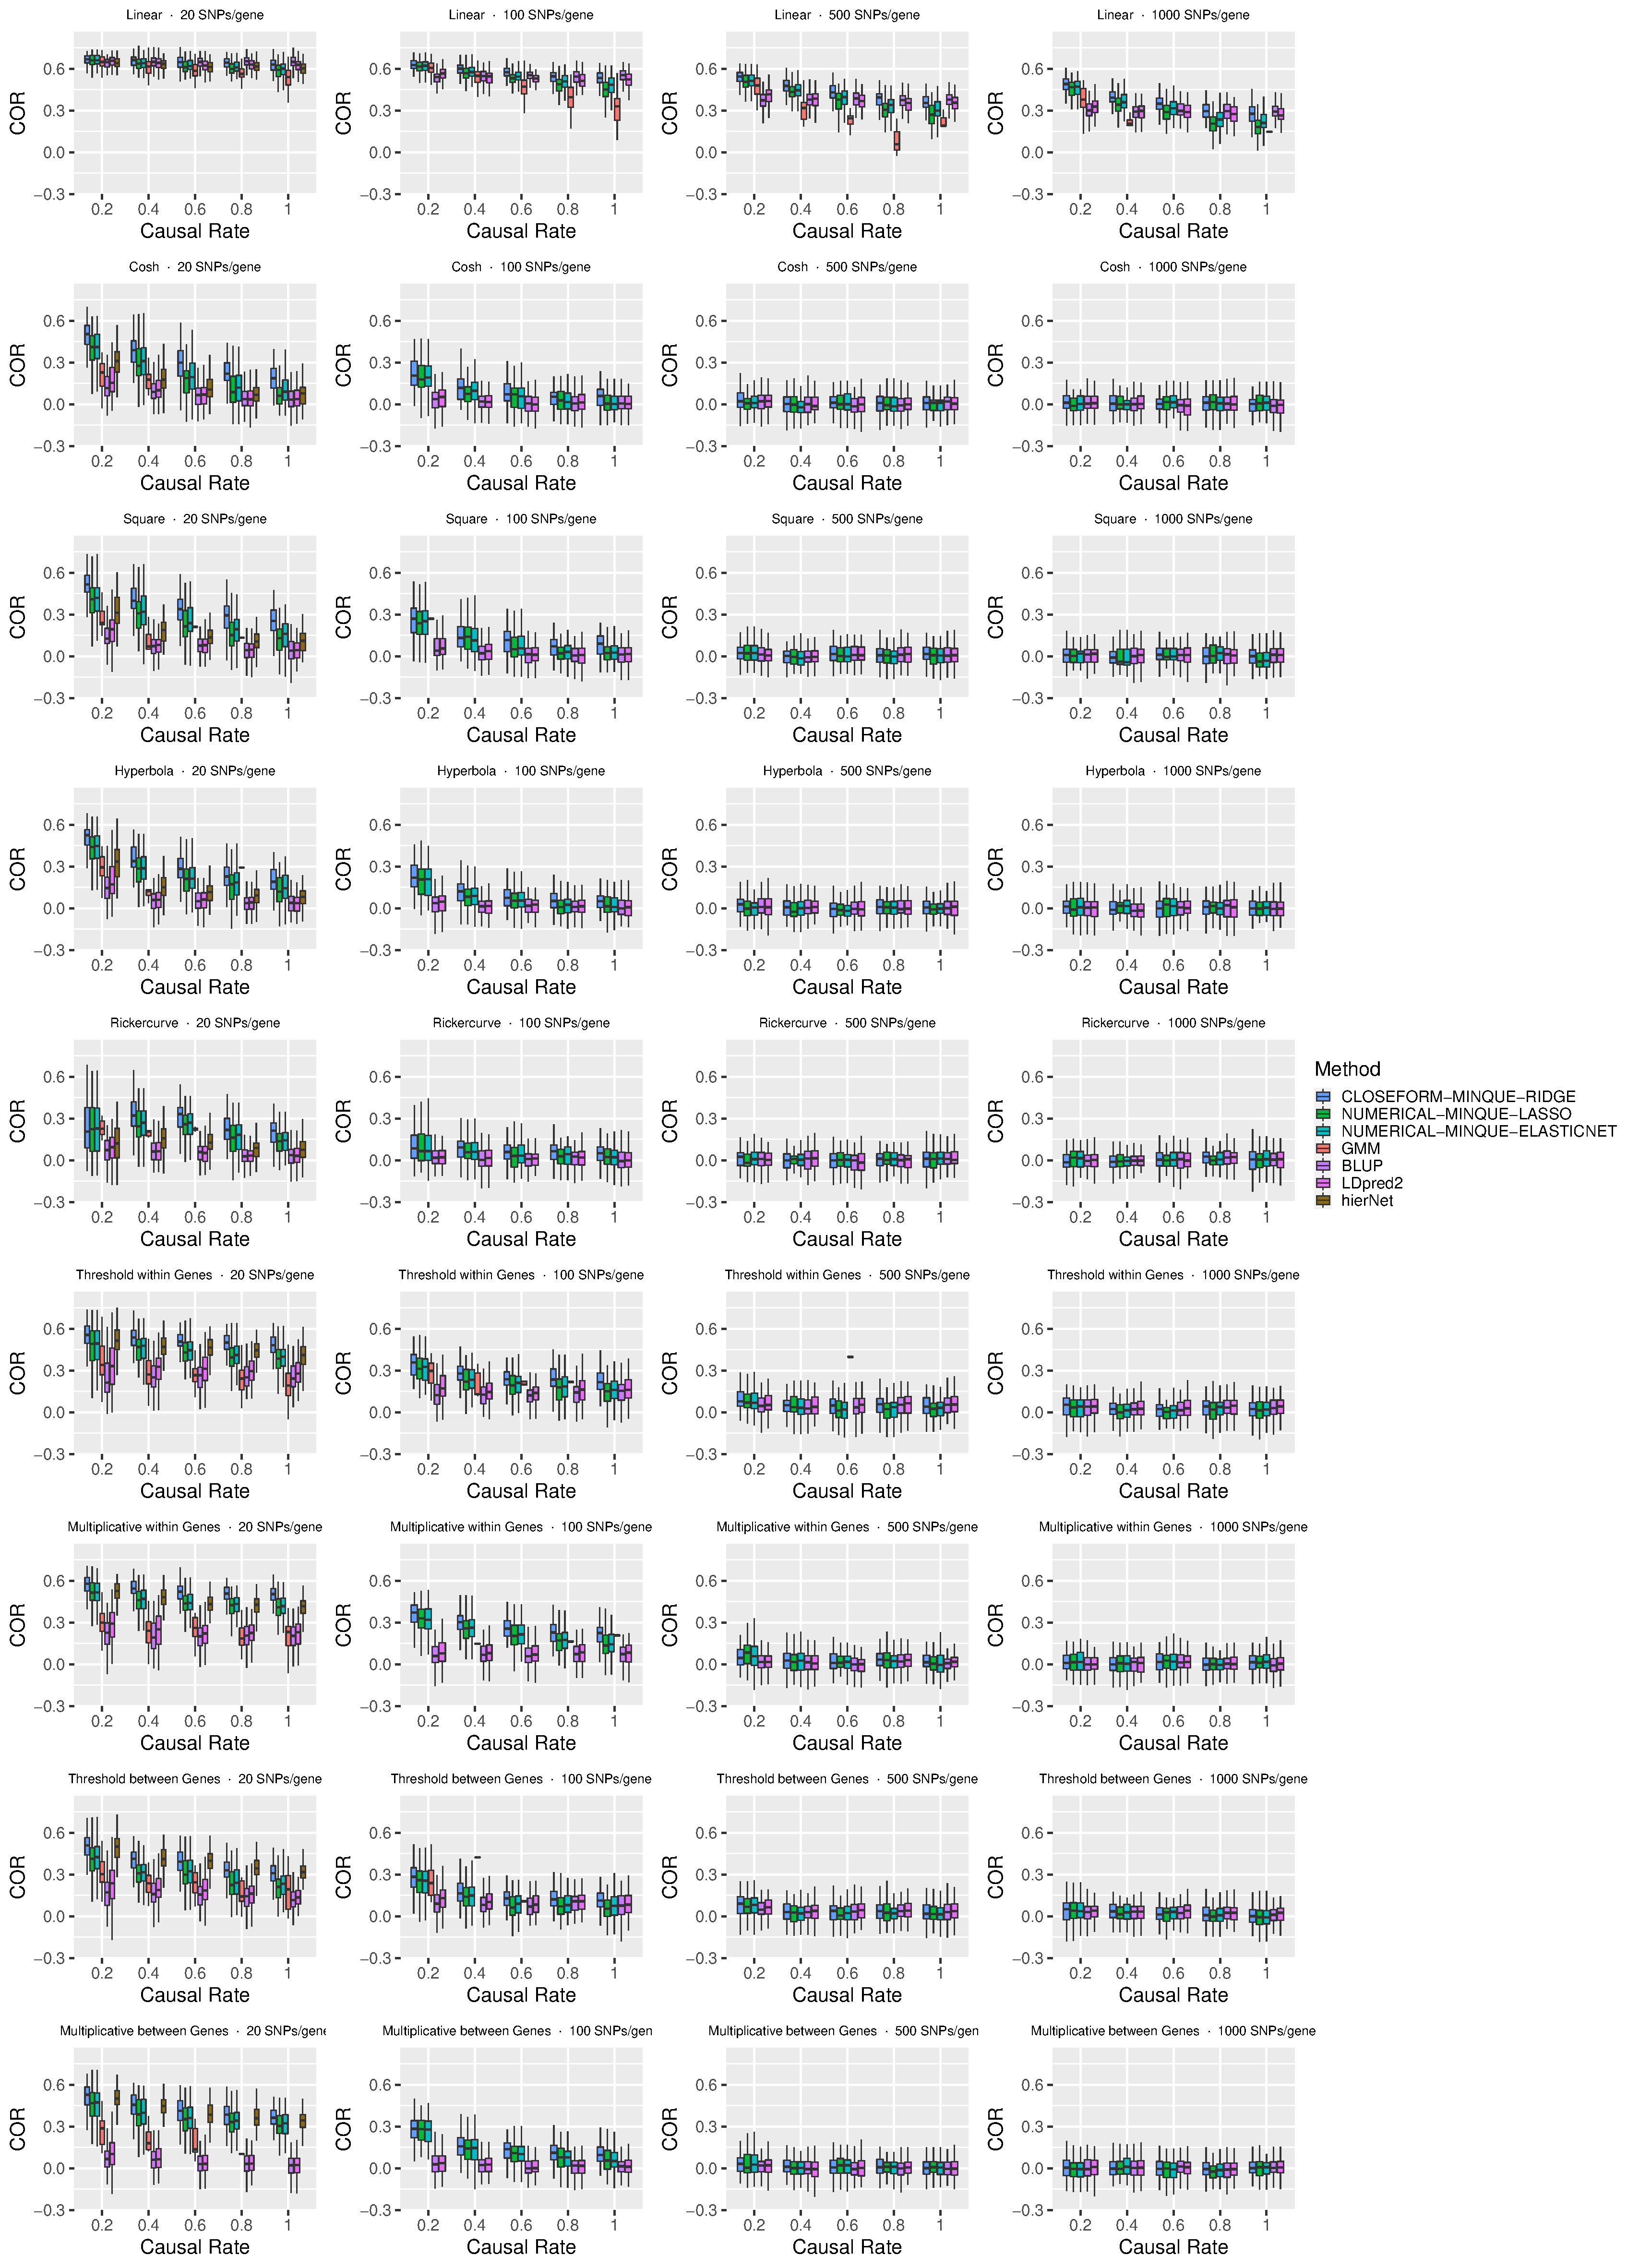
\includegraphics[height=0.9\textheight]{sim_h2_0.5_correlation.pdf}
  \caption{Out-of-sample prediction accuracy across the full simulation design
  at heritability $h^2=0.5$.  Rows are the nine genetic architectures: five
  link functions applied to the regional genetic score (linear, cosh, square,
  hyperbola, Ricker curve) and four interaction mechanisms (thresholded and
  multiplicative products, formed within genes and between genes).  Columns are
  SNP density, at 20, 100, 500 and 1000 SNPs per gene across ten genes.  Within
  each panel the horizontal axis is the causal rate, the proportion of SNPs in a
  causal gene that carry an effect.  Boxes summarise the correlation between
  predicted and observed phenotype in the held-out set over 100 replicates;
  outliers are suppressed and the vertical range is shared across all panels so
  that they are directly comparable.  Genotypes are real, drawn as contiguous
  windows from UK Biobank so that the simulated regions carry authentic linkage
  disequilibrium.  hierNet appears only in the 20 SNPs per gene column: above that
  density the number of pairwise terms exceeds the 32-bit indexing limit of its
  compiled back end.  GMM contributes usable fits in only 10.1\% of cases,
  because its one-standard-error penalty rule frequently shrinks the genetic
  component to a constant; the remaining methods contribute between 76\% and
  100\%.}
  \label{fig:sim-h2-05}
\end{figure}


% ---------------------------------------------------------------- Figure 3
\begin{figure}[p]
  \centering
  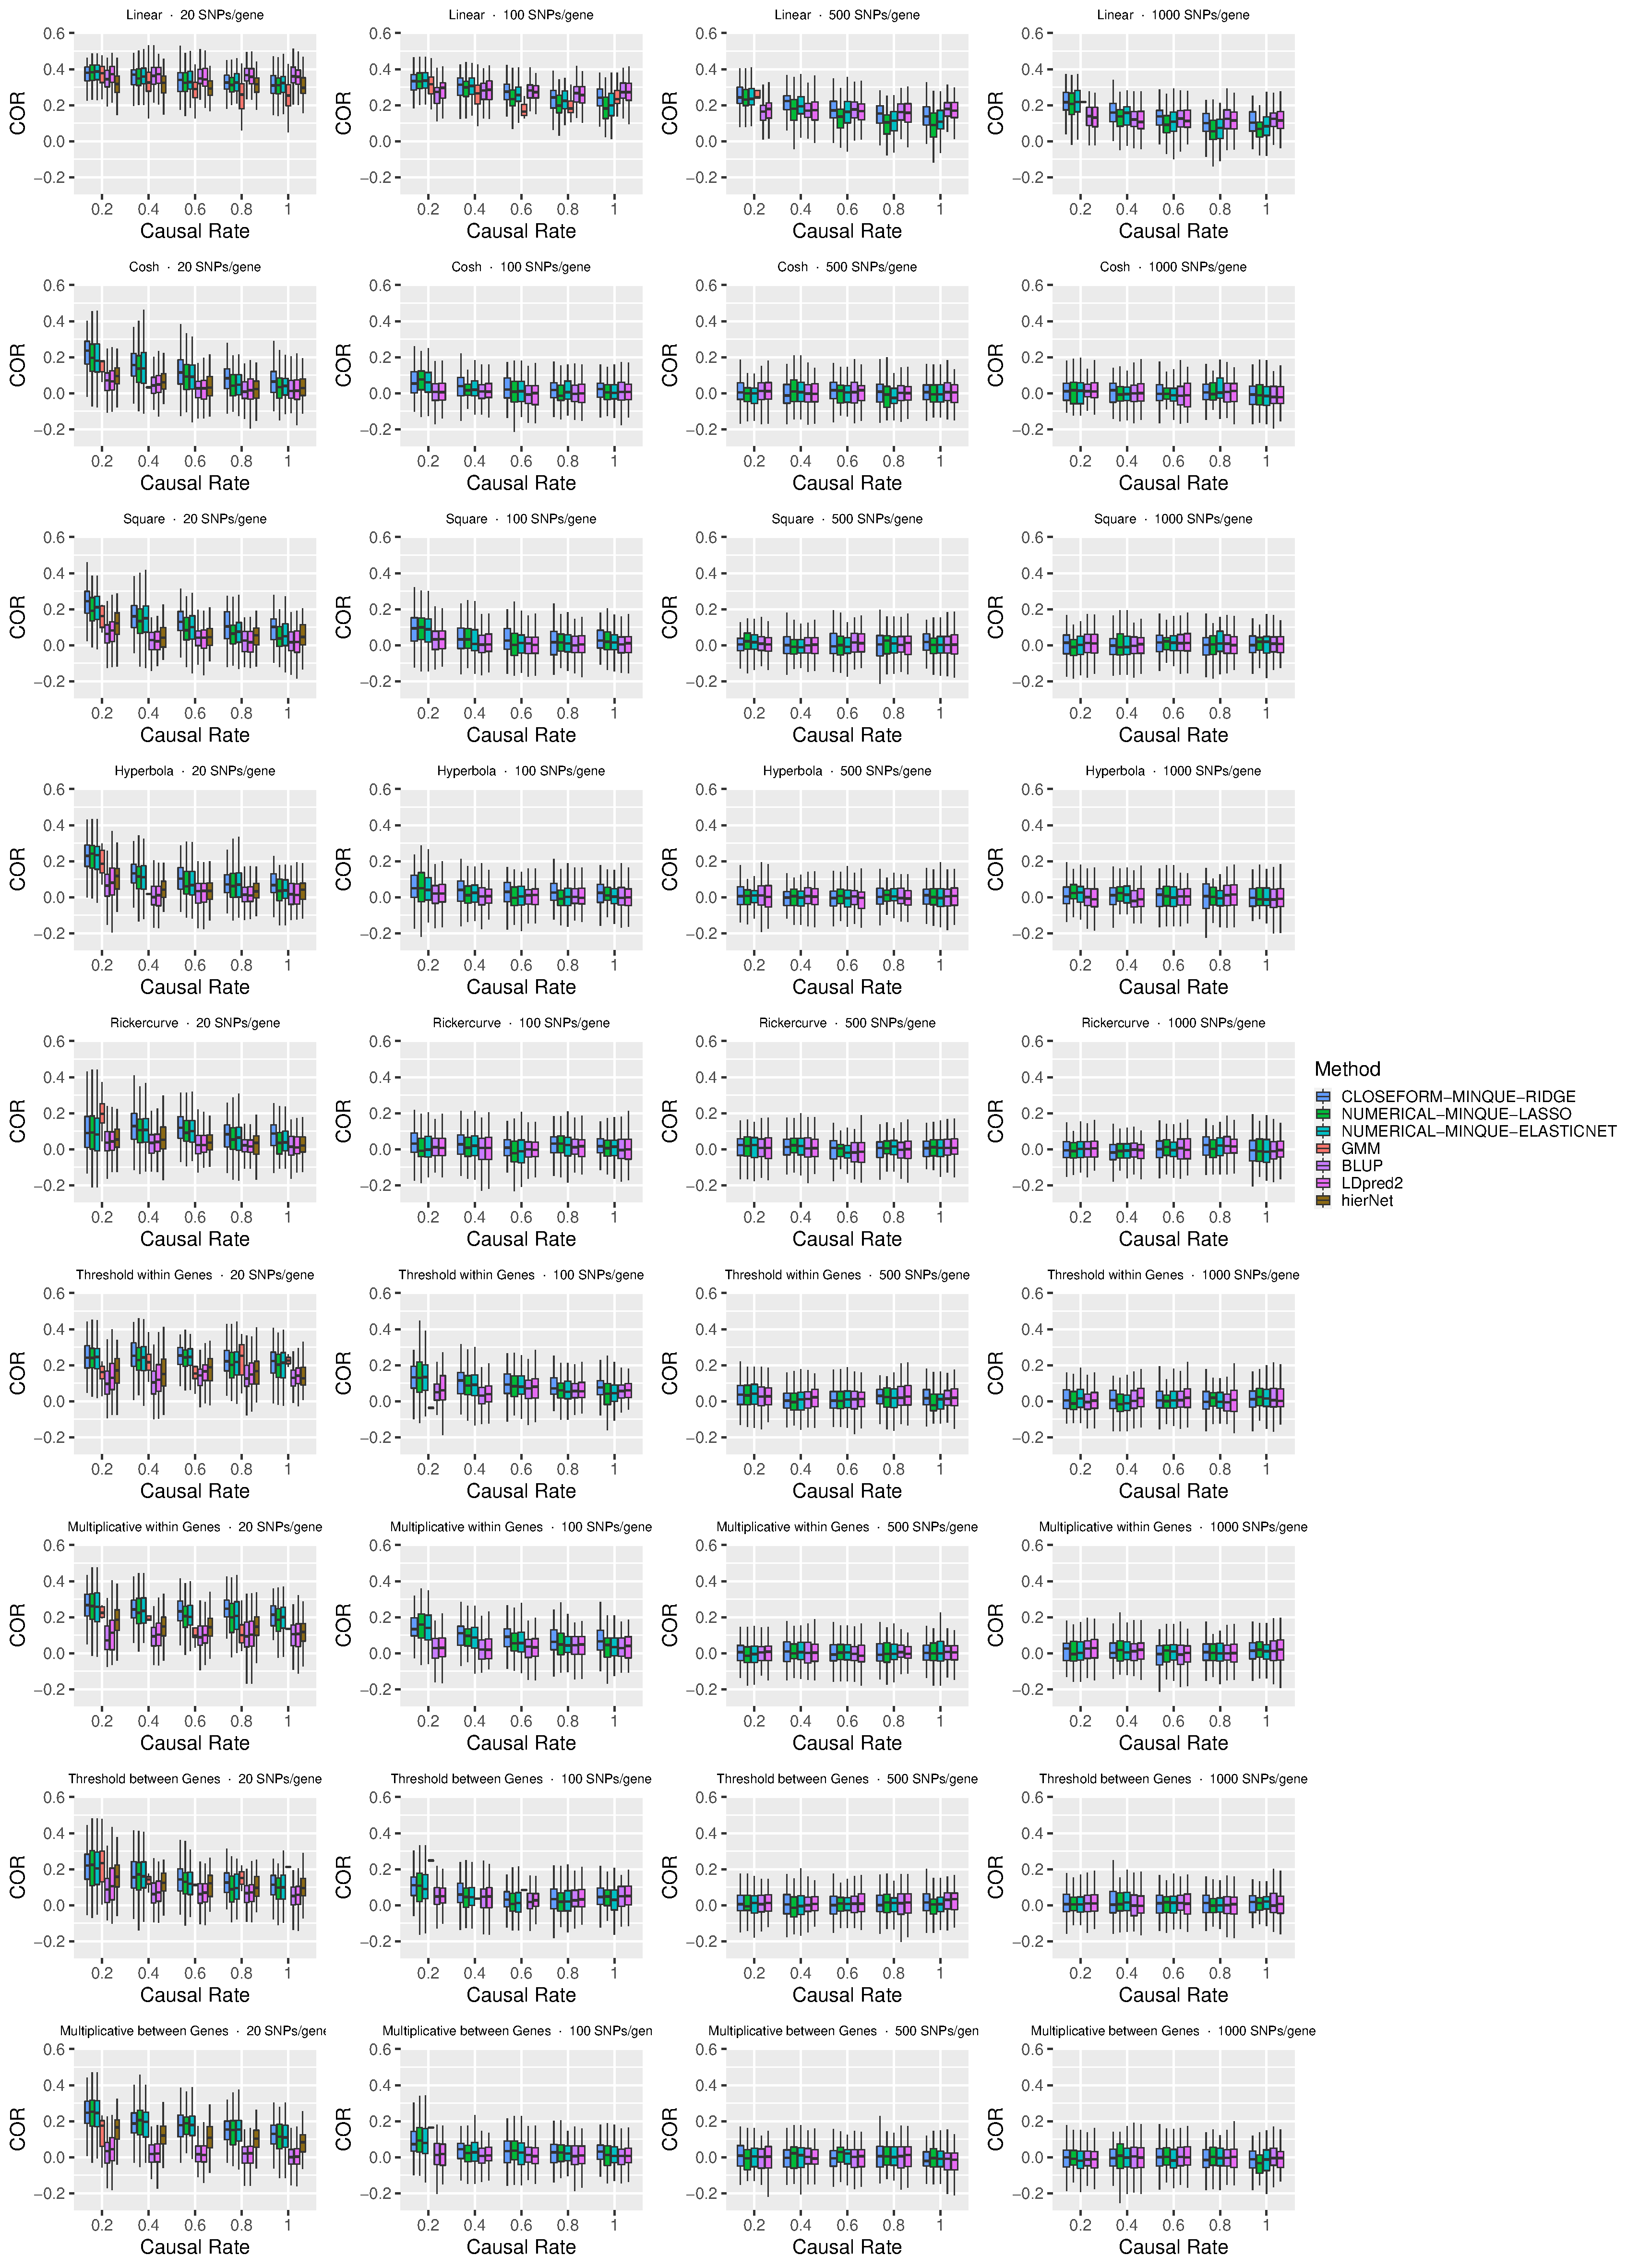
\includegraphics[height=0.9\textheight]{sim_h2_0.2_correlation.pdf}
  \caption{Out-of-sample prediction accuracy across the same simulation design
  at the lower heritability $h^2=0.2$.  Layout, axes, replication and genotype
  source are identical to Figure~\ref{fig:sim-h2-05}; only the proportion of
  phenotypic variance attributable to genetics differs.  Accuracy falls for
  every method, and the ordering among methods is broadly preserved, indicating
  that the comparison is not an artefact of a favourable signal-to-noise ratio.
  Collapse is more frequent at this heritability: GMM contributes usable fits in
  3.9\% of cases, against 72.6\% for the lasso-penalized and 85.2\% for the
  elastic-net-penalized numerical MINQUE, and 100\% for the closed-form
  estimator.}
  \label{fig:sim-h2-02}
\end{figure}


% ---------------------------------------------------------------- Figure 4
\begin{figure}[htbp]
  \centering
  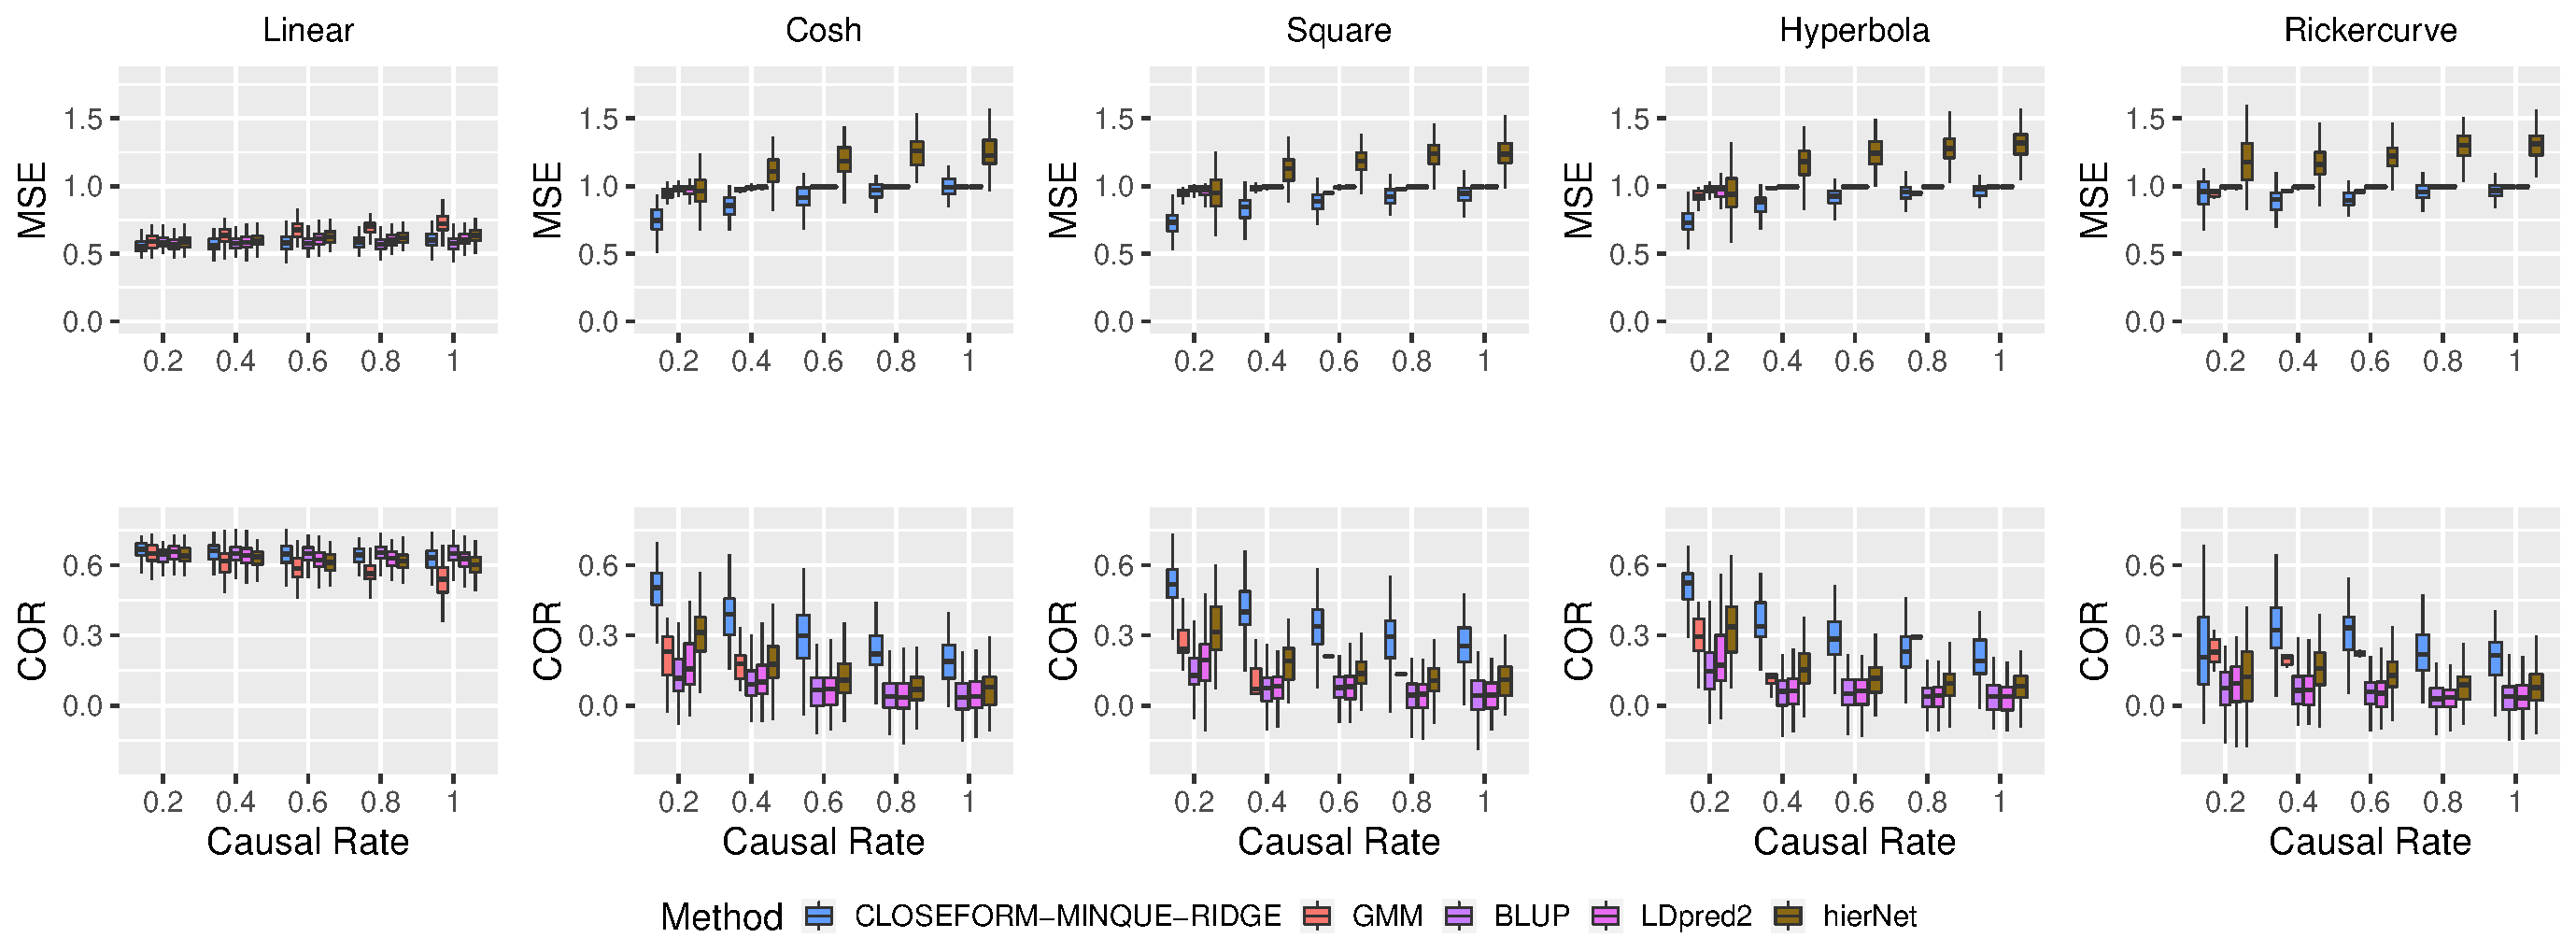
\includegraphics[width=\textwidth]{sim_h2_0.5_nonlinear_baselines_P20.pdf}
  \caption{Comparison of the proposed estimator with external baselines under
  the five nonlinear architectures, at $h^2=0.5$ and 20 SNPs per gene across
  ten genes.  The upper row reports mean squared prediction error and the lower
  row the correlation between predicted and observed phenotype, both in the
  held-out set over 100 replicates; the horizontal axis is the causal rate.
  Vertical ranges are shared across each row so the columns can be compared.
  The density of 20 SNPs per gene is the one at which all five methods can be
  evaluated: hierNet cannot be fitted above it.  GMM boxes summarise 598 of
  2500 fits, the remainder having collapsed to a constant genetic prediction;
  the other four methods contribute all 2500.}
  \label{fig:sim-nonlinear-baselines}
\end{figure}


% ---------------------------------------------------------------- Figure 5
\begin{figure}[htbp]
  \centering
  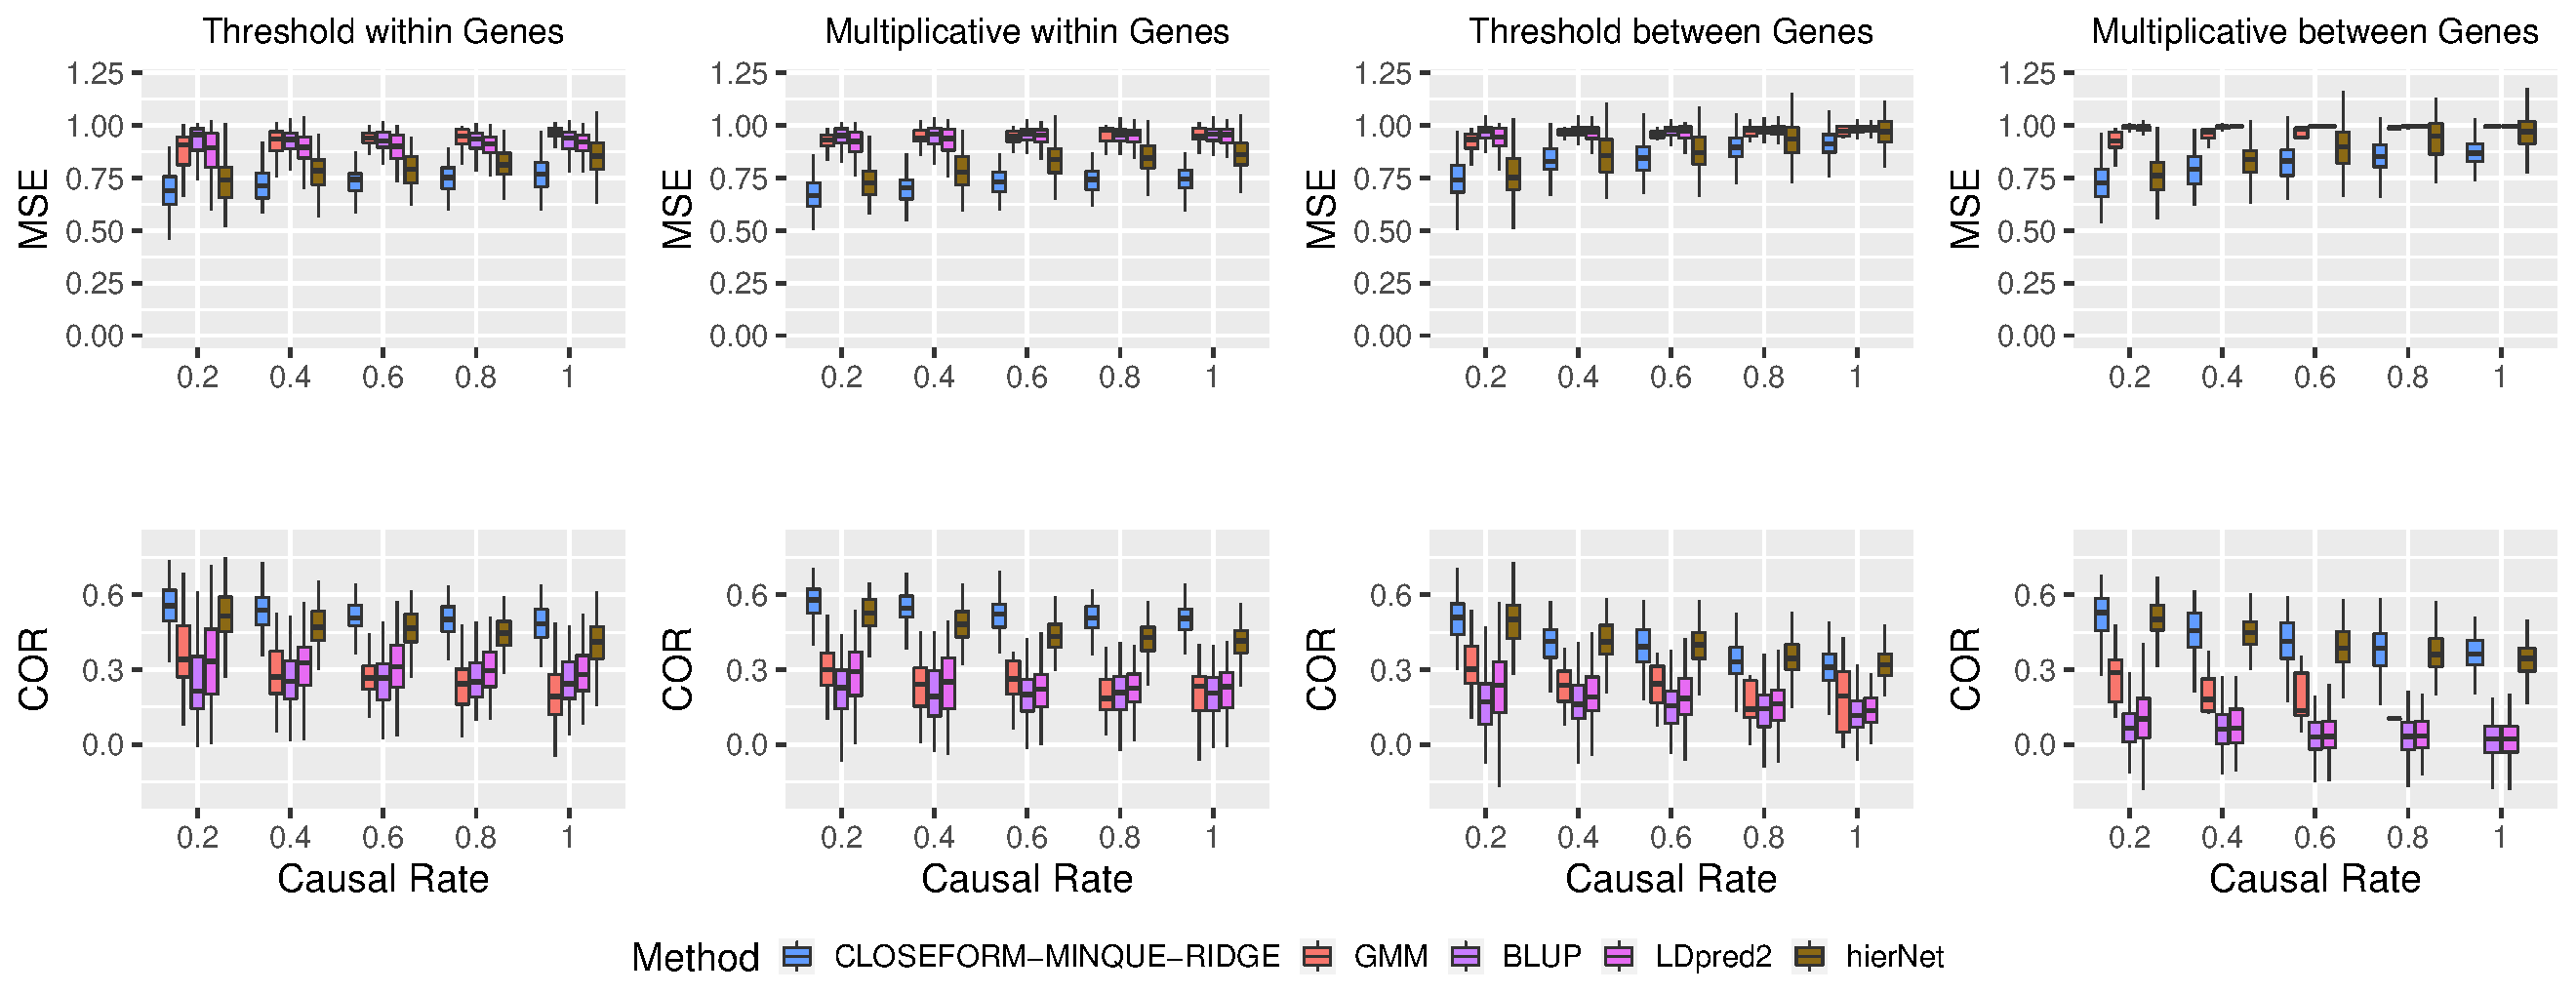
\includegraphics[width=\textwidth]{sim_h2_0.5_interaction_baselines_P20.pdf}
  \caption{Comparison of the proposed estimator with external baselines under
  the four interaction architectures, at $h^2=0.5$ and 20 SNPs per gene.
  Interaction phenotypes are built from products of causal SNP pairs, either
  drawn within a single causal gene or across distinct causal genes, and either
  passed through a threshold at zero or left multiplicative.  Rows, axes,
  replication and vertical ranges follow Figure~\ref{fig:sim-nonlinear-baselines}.
  These architectures are the ones the interaction kernel basis is designed to
  capture, and the comparison against hierNet is the like-for-like contrast:
  both models span the same class of degree-two polynomials, but represent it
  differently, PKNN through kernel products under a block-exchangeable Gaussian
  prior and hierNet through explicit cross-product terms under a sparsity and
  heredity constraint.  GMM boxes summarise 440 of 2000 fits; the other methods
  contribute all 2000.}
  \label{fig:sim-interaction-baselines}
\end{figure}


% ---------------------------------------------------------------- Figure 6
\begin{figure}[htbp]
  \centering
  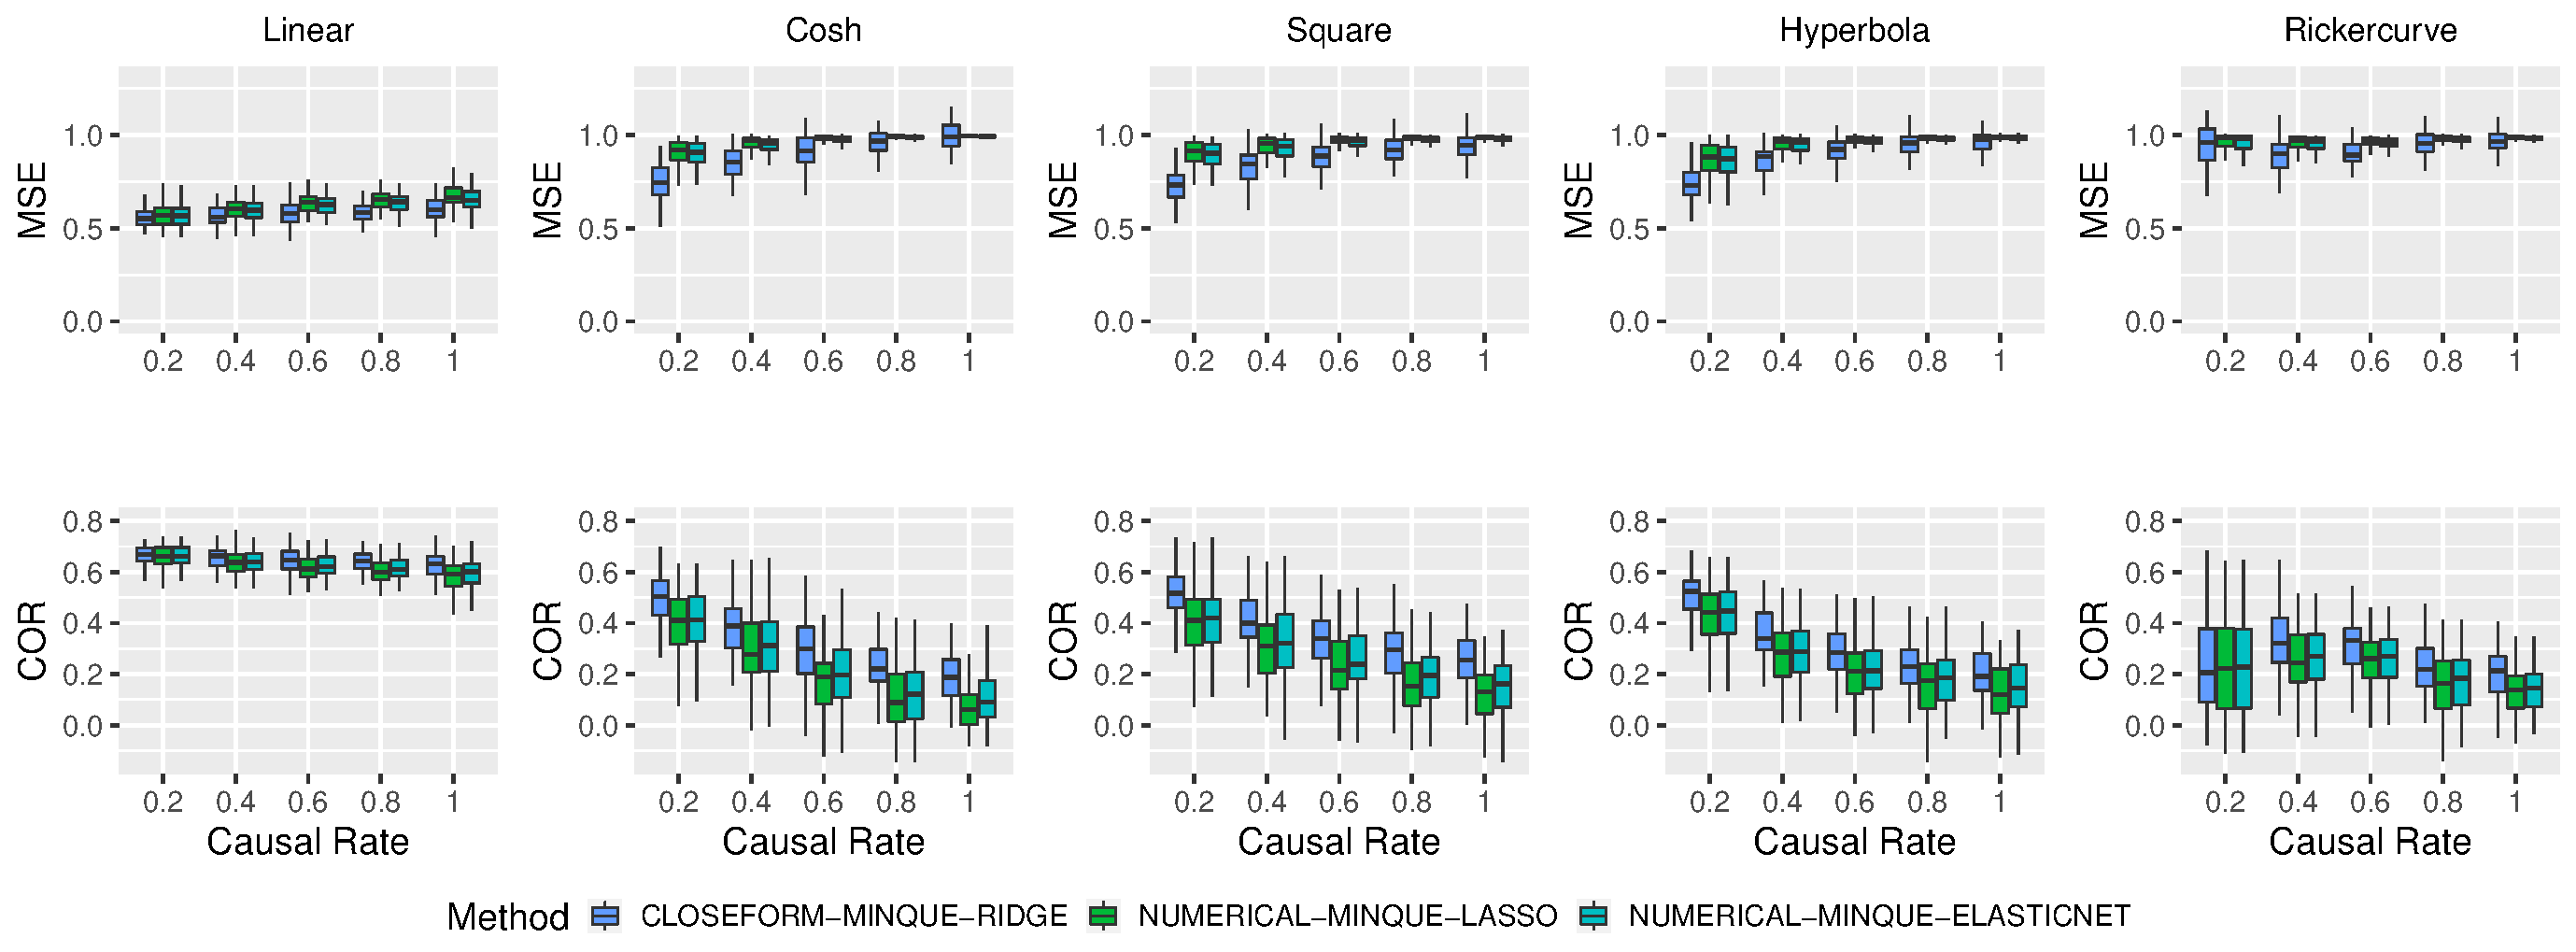
\includegraphics[width=\textwidth]{sim_h2_0.5_nonlinear_minque_P20.pdf}
  \caption{Effect of the penalty on variance component selection, under the five
  nonlinear architectures at $h^2=0.5$ and 20 SNPs per gene.  The three methods
  differ only in how the MINQUE variance components are penalized: a closed-form
  ridge solution, and numerical solutions under a lasso and an elastic-net
  penalty.  Rows, axes, replication and vertical ranges follow
  Figure~\ref{fig:sim-nonlinear-baselines}.  This comparison isolates why the
  ridge penalty is preferred in this setting.  The kernel components are
  strongly correlated with one another, so the sparse penalties select unstably
  among near-equivalent components rather than discarding genuinely null ones,
  and they fail to return a usable fit in 5.2\% (lasso) and 3.4\% (elastic net)
  of replicates, against none for the ridge solution.}
  \label{fig:sim-nonlinear-minque}
\end{figure}


% ---------------------------------------------------------------- Figure 7
\begin{figure}[htbp]
  \centering
  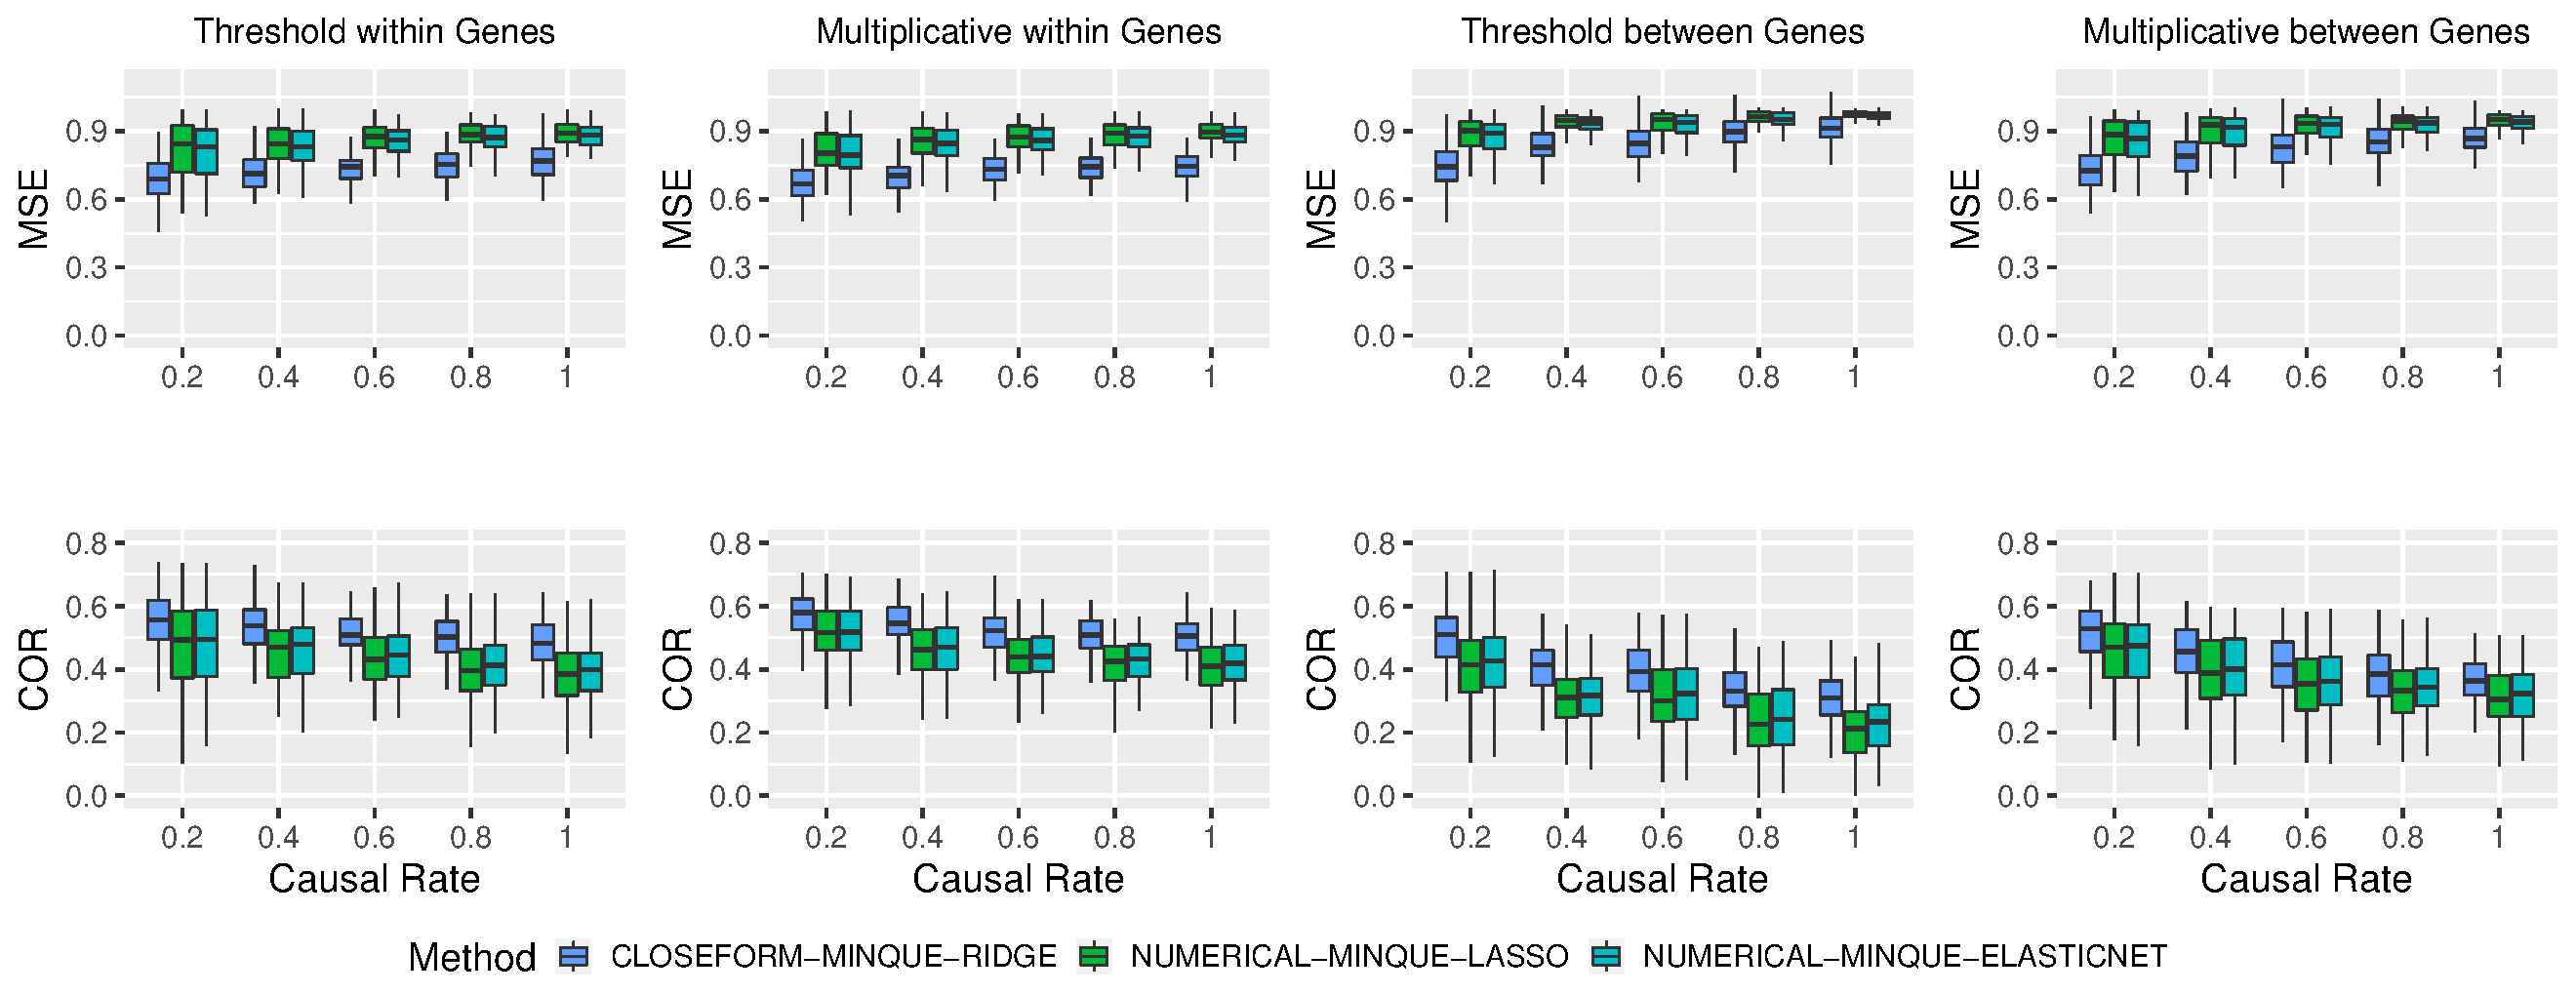
\includegraphics[width=\textwidth]{sim_h2_0.5_interaction_minque_P20.pdf}
  \caption{Effect of the penalty on variance component selection, under the four
  interaction architectures at $h^2=0.5$ and 20 SNPs per gene.  Methods, rows,
  axes, replication and vertical ranges follow
  Figure~\ref{fig:sim-nonlinear-minque}.  With the interaction basis the number
  of components grows from twelve to 67 while the sample size is unchanged, so
  the components are both more numerous and more collinear; the ridge solution
  remains stable across all 2000 replicates, while the sparse penalties again
  fail on a small fraction.}
  \label{fig:sim-interaction-minque}
\end{figure}


% ------------------------------------------------------ Figures 8 and 9
% How many candidate genes to supply.  Two figures, nonlinear and interaction.
\begin{figure}[htbp]
  \centering
  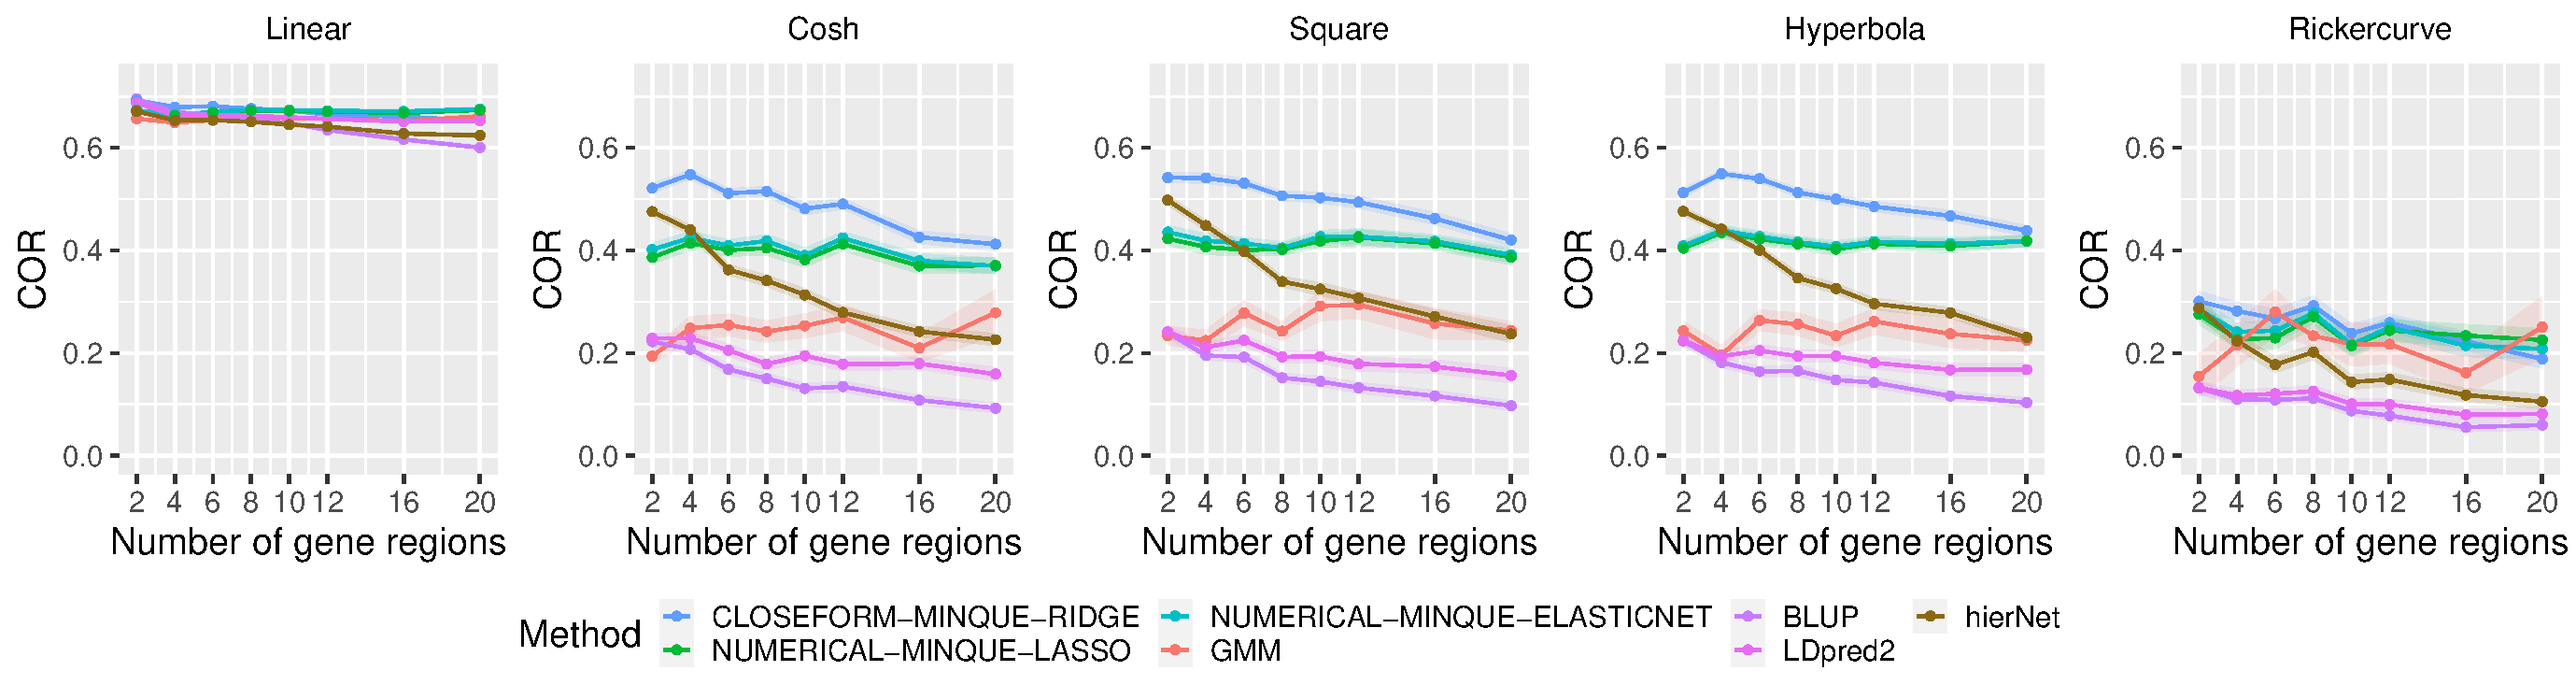
\includegraphics[width=\textwidth]{sim_ngene_nonlinear_P20.pdf}
  \caption{Effect of the number of candidate genes supplied to the model, under the
  five nonlinear architectures at $h^2=0.5$ and 20 SNPs per gene.  In every panel
  exactly two regions carry causal variants while the number of regions given to the
  model grows from two to twenty, so the horizontal axis measures the cost of
  including uninformative genes rather than a change in the amount of signal.  Two
  regions is the oracle, at which only the informative genes are supplied; twenty is
  the ceiling imposed by placing one region per chromosome, and supplies eighteen
  uninformative regions alongside the two causal ones.  Points are mean out-of-sample
  correlation over 100 replicates and bands are one standard error.  The proposed
  estimator degrades gracefully, retaining 97\% of its oracle accuracy with eight
  regions supplied, 93\% with twelve and 82\% with twenty, whereas hierNet retains
  55\% and gBLUP 52\% over the same range: the explicit interaction search pays
  quadratically for null predictors, and a single additive relationship matrix
  dilutes the signal across every region it pools.  The sparse penalties are the most
  stable of all, retaining 95\% and 92\%, though from a lower starting point.  The
  practical implication is that an inclusive candidate list costs the proposed method
  little.  Note that GMM returns a usable fit in only about a third of replicates at
  every region count, so its curve summarises a subset selected for not having
  collapsed and its apparent improvement should not be read as robustness.}
  \label{fig:sim-ngene-nonlinear}
\end{figure}


\begin{figure}[htbp]
  \centering
  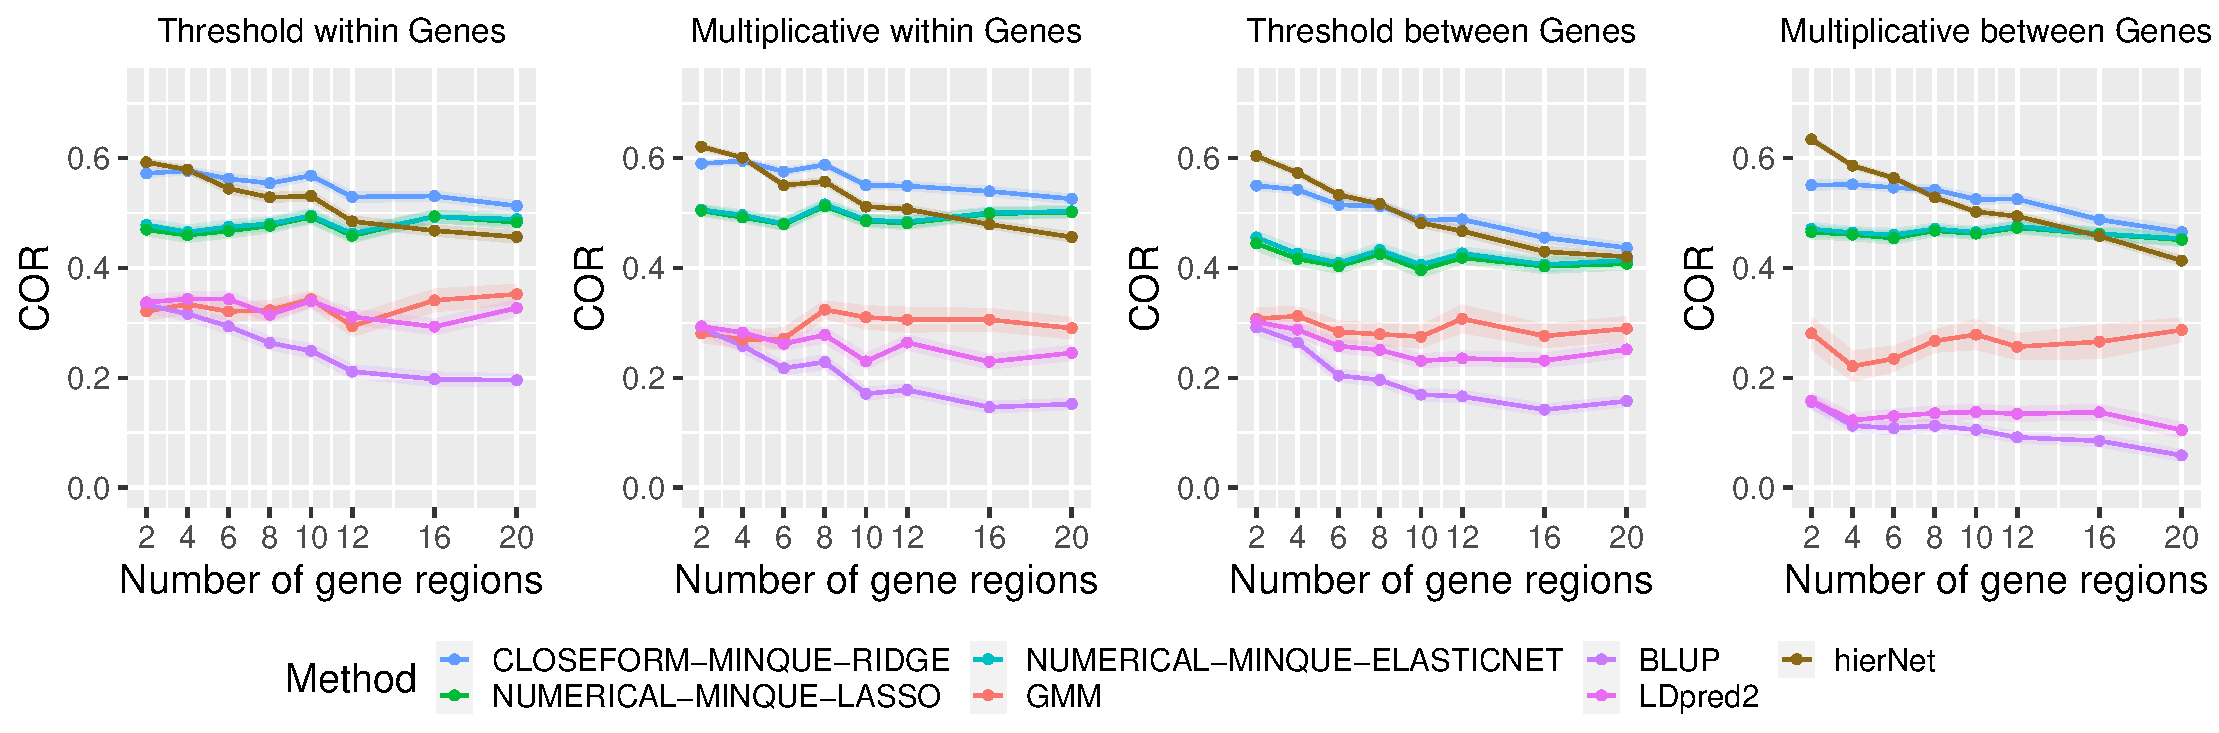
\includegraphics[width=\textwidth]{sim_ngene_interaction_P20.pdf}
  \caption{Effect of the number of candidate genes supplied to the model, under the
  four interaction architectures at $h^2=0.5$ and 20 SNPs per gene.  Design, axes and
  replication follow Figure~\ref{fig:sim-ngene-nonlinear}, and the vertical range is
  shared between the two figures so they can be read against each other.  These are
  the architectures for which the interaction kernel basis is intended, and the
  ordering of the two interaction models reverses across the axis: hierNet is the more
  accurate at the oracle, where only two genes are supplied and its pairwise search is
  small (0.613 against 0.566), but it loses ground steadily and the proposed estimator
  is ahead from six regions onward, by 0.485 against 0.437 at twenty.  Retention over
  the same range is 86\% for the proposed estimator against 71\% for hierNet and 51\%
  for gBLUP.  The comparison therefore does not show that the kernel representation
  models pairwise interaction better than an explicit search does; it shows that the
  two span the same class of effects while the kernel form is far less sensitive to the
  presence of uninformative genes, which is the situation a candidate-gene analysis
  actually faces.  As in Figure~\ref{fig:sim-ngene-nonlinear}, GMM is usable in only
  about a third of replicates.}
  \label{fig:sim-ngene-interaction}
\end{figure}


% ---------------------------------------------------- Figures 10 and 11
% Within-region sparsity.  Two figures, nonlinear and interaction.
\begin{figure}[htbp]
  \centering
  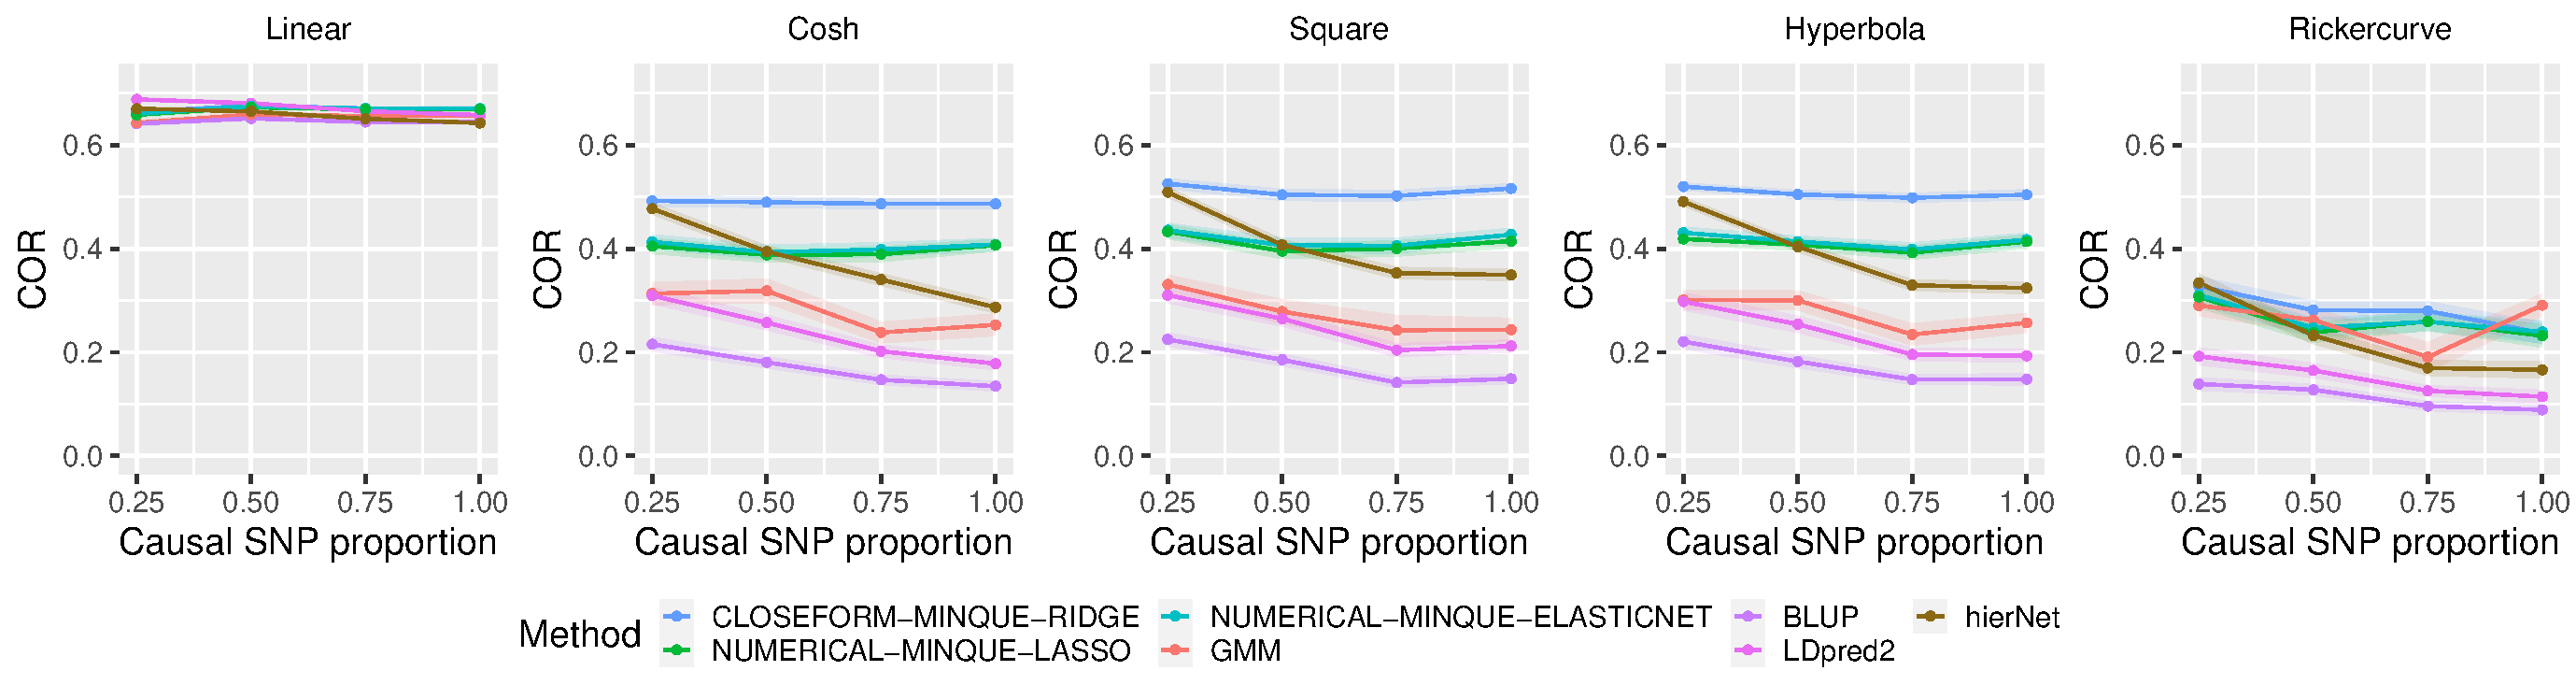
\includegraphics[width=\textwidth]{sim_sparse_nonlinear.pdf}
  \caption{Effect of within-region sparsity under the five nonlinear
  architectures, at $h^2=0.5$, 20 SNPs per gene, ten regions and a causal rate of
  0.2, so that two of the ten regions carry signal.  The horizontal axis is the
  proportion of the twenty SNPs inside each causal region that carry an effect:
  at 0.25 only five do and the remaining fifteen are noise within a causal
  region, while at 1.00 every SNP is causal, which reproduces the design used
  elsewhere in the paper and agrees with it to within 0.002.  Points are mean
  out-of-sample correlation over 100 replicates and bands are one standard
  error.  The proposed estimator is insensitive to sparsity, attaining 0.506 at a
  proportion of 0.25 against 0.483 at 1.00, because the penalty acts on
  region-level variance components rather than on individual SNP effects and a
  region carrying even a few causal variants has a non-zero component.  hierNet
  moves in the opposite direction, from 0.496 to 0.354, as a denser causal set
  enlarges the pairwise search it must perform.  GMM returns a usable fit in
  about 42\% of replicates here, so its curve summarises a selected subset.}
  \label{fig:sim-sparse-nonlinear}
\end{figure}


\begin{figure}[htbp]
  \centering
  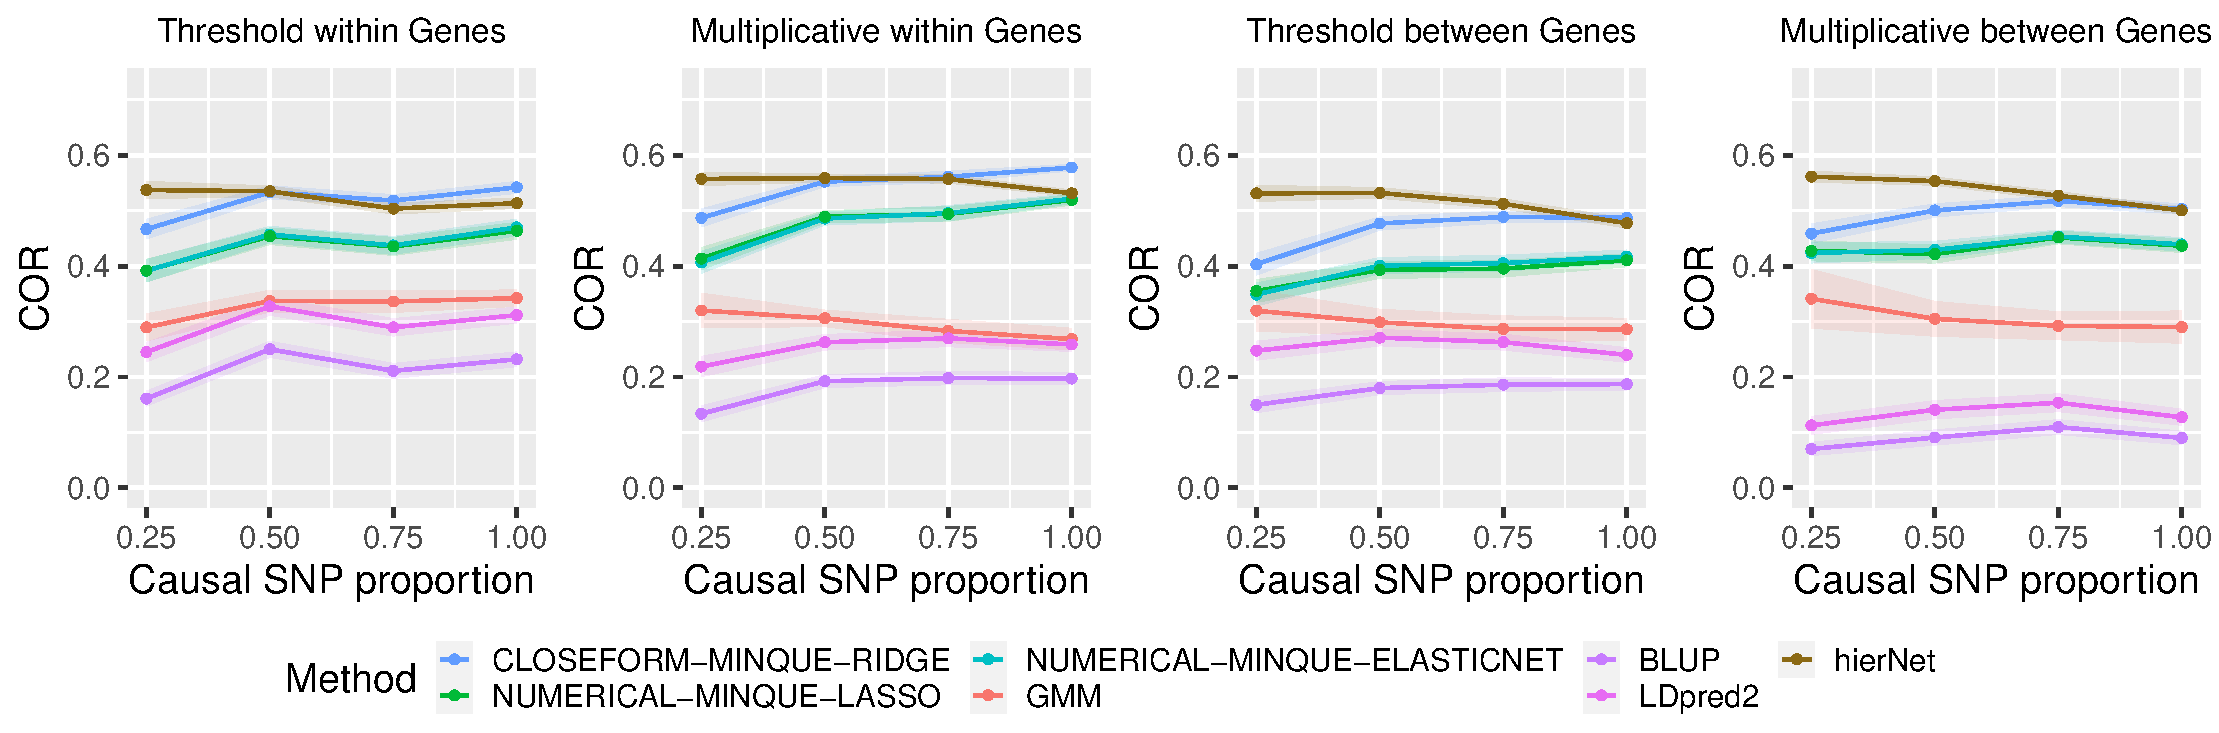
\includegraphics[width=\textwidth]{sim_sparse_interaction.pdf}
  \caption{Effect of within-region sparsity under the four interaction
  architectures.  Design, axes, replication and the shared vertical range follow
  Figure~\ref{fig:sim-sparse-nonlinear}.  Here the dependence on sparsity is
  reversed for both interaction models and their ordering changes across the
  axis: the proposed estimator improves with a denser causal set, from 0.454 at a
  proportion of 0.25 to 0.528 at 1.00, whereas hierNet declines from 0.547 to
  0.506 and is the more accurate of the two at the sparsest setting.  This is the
  expected behaviour, since a small number of causal variants produces few
  interacting pairs, which is precisely the regime an explicit pairwise search is
  designed for, while the region-level kernel gains as signal becomes distributed
  across the region.  As in Figure~\ref{fig:sim-sparse-nonlinear}, GMM is usable
  in a minority of replicates, here about 29\%.}
  \label{fig:sim-sparse-interaction}
\end{figure}



% ---------------------------------------------------- Figures 12 and 13
% Sample size.  Two figures, nonlinear and interaction.
\begin{figure}[htbp]
  \centering
  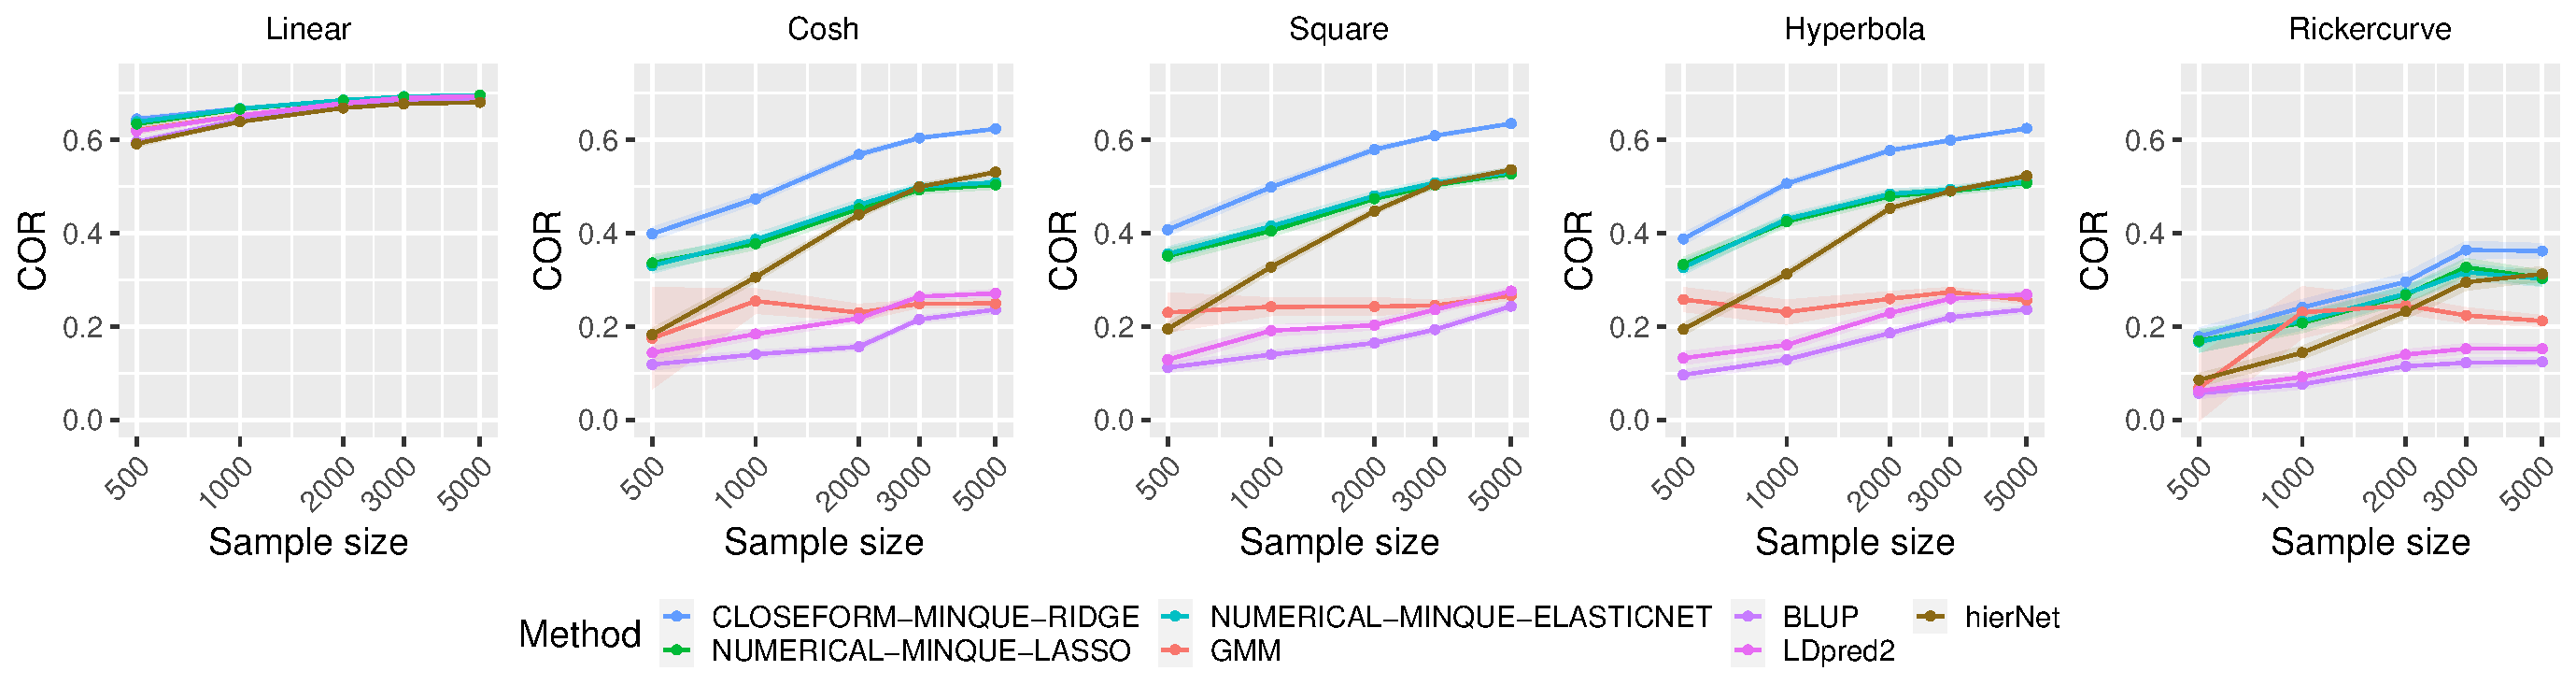
\includegraphics[width=\textwidth]{sim_nvary_nonlinear.pdf}
  \caption{Effect of sample size under the five nonlinear architectures, at
  $h^2=0.5$, 20 SNPs per gene, ten regions and a causal rate of 0.2.  The
  horizontal axis is the total sample size on a logarithmic scale, split into
  training and testing sets by $n_{\text{test}} = \max(100, 0.2N)$, the same rule
  used in the computational study, so that $N=1000$ is the 800/200 split used
  throughout the paper.  Points are mean out-of-sample correlation over 100
  replicates and bands are one standard error.  All methods improve with sample
  size, but they do not converge: the advantage of the proposed estimator over the
  additive benchmarks widens, from 0.403 against 0.196 for gBLUP at $N=500$ to
  0.588 against 0.306 at $N=5000$.  hierNet gains the most of any method over this
  range, from 0.249 to 0.517, which is consistent with an explicit pairwise search
  having the most parameters to estimate and therefore the most to gain from
  additional samples, but it remains well below the proposed estimator at every
  sample size.  GMM gains least, from 0.270 to 0.334.}
  \label{fig:sim-nvary-nonlinear}
\end{figure}


\begin{figure}[htbp]
  \centering
  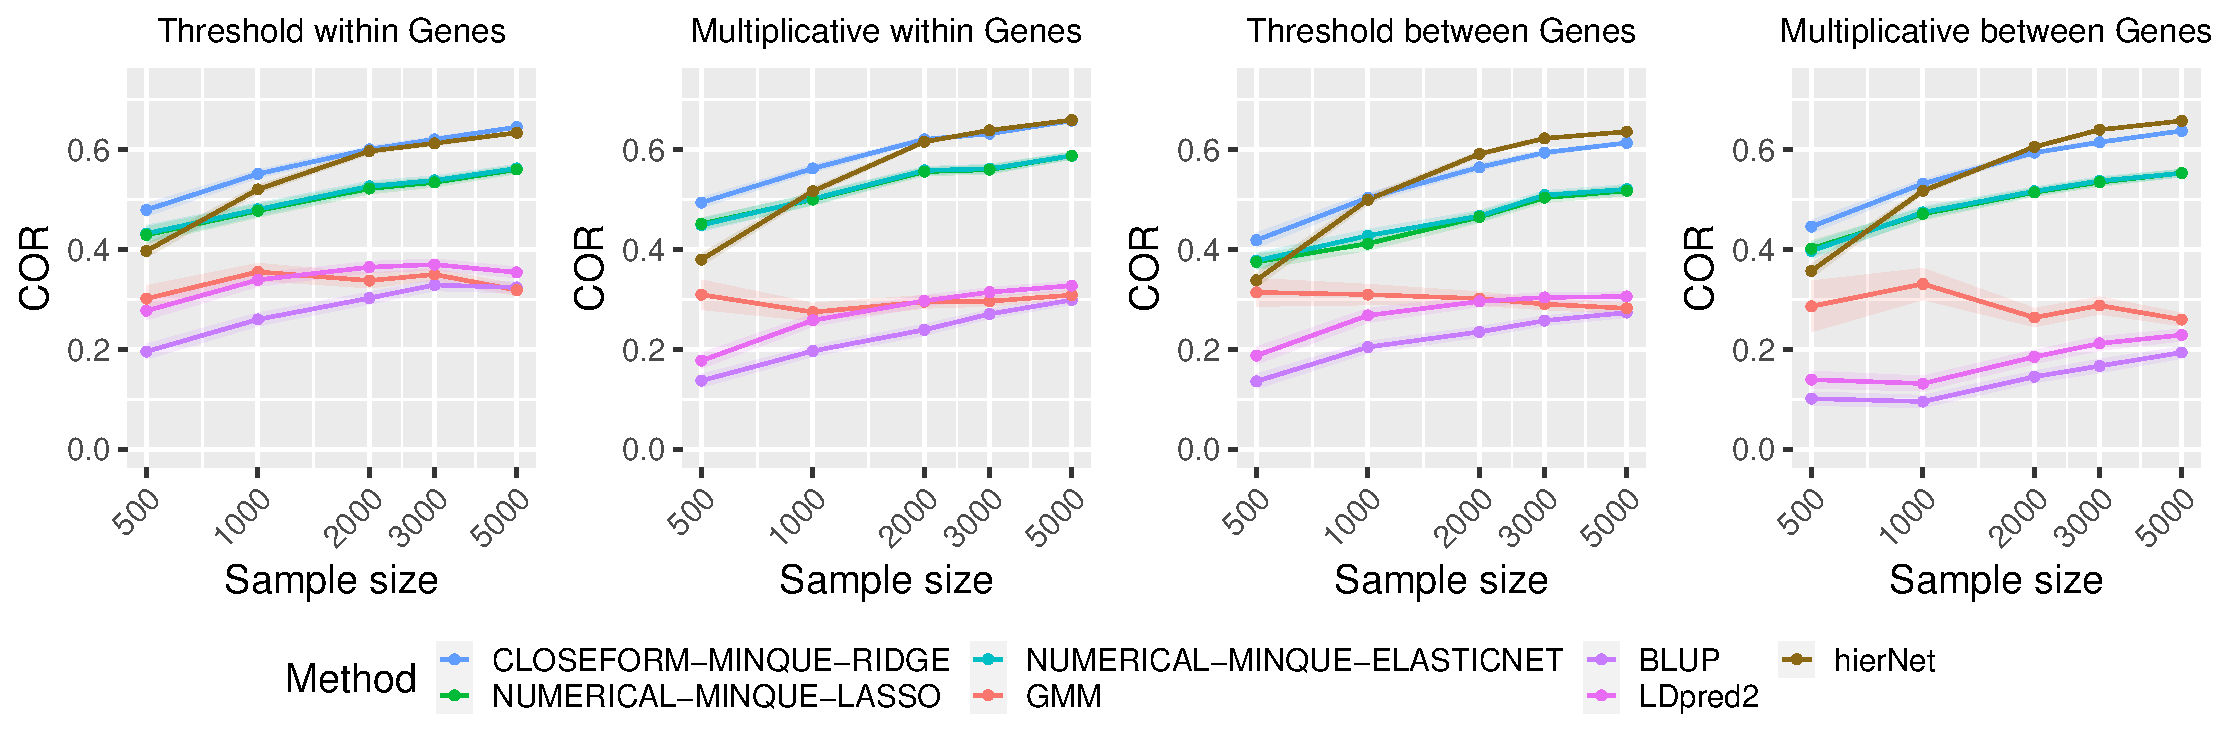
\includegraphics[width=\textwidth]{sim_nvary_interaction.pdf}
  \caption{Effect of sample size under the four interaction architectures.
  Design, axes, replication and the shared vertical range follow
  Figure~\ref{fig:sim-nvary-nonlinear}.  The proposed estimator improves from
  0.459 at $N=500$ to 0.639 at $N=5000$ and again separates from the additive
  benchmarks rather than converging with them, while GMM is the one method that
  does not benefit from a larger sample here, declining slightly from 0.303 to
  0.292.  The ordering of the two interaction models reverses with sample size:
  pairing replicates within scenario, the proposed estimator is ahead by 0.091 at
  $N=500$ and 0.024 at $N=1000$, and behind by 0.007, 0.013 and 0.008 at $N=2000$,
  3000 and 5000 (paired $t$-test on 400 pairs, $p<0.001$ at every level).  The
  margins beyond the crossover are small but systematic, and the direction is what
  one would expect: when the generating model is exactly pairwise, estimating
  those terms explicitly becomes more efficient than a kernel prior once the
  sample is large enough to support it.  The advantage of the kernel
  representation lies instead in the smooth nonlinear architectures of
  Figure~\ref{fig:sim-nvary-nonlinear}, at smaller sample sizes, and in
  robustness to uninformative genes (Figure~\ref{fig:sim-ngene-interaction}).}
  \label{fig:sim-nvary-interaction}
\end{figure}


% --------------------------------------------------------------- Figure 14
\begin{figure}[htbp]
  \centering
  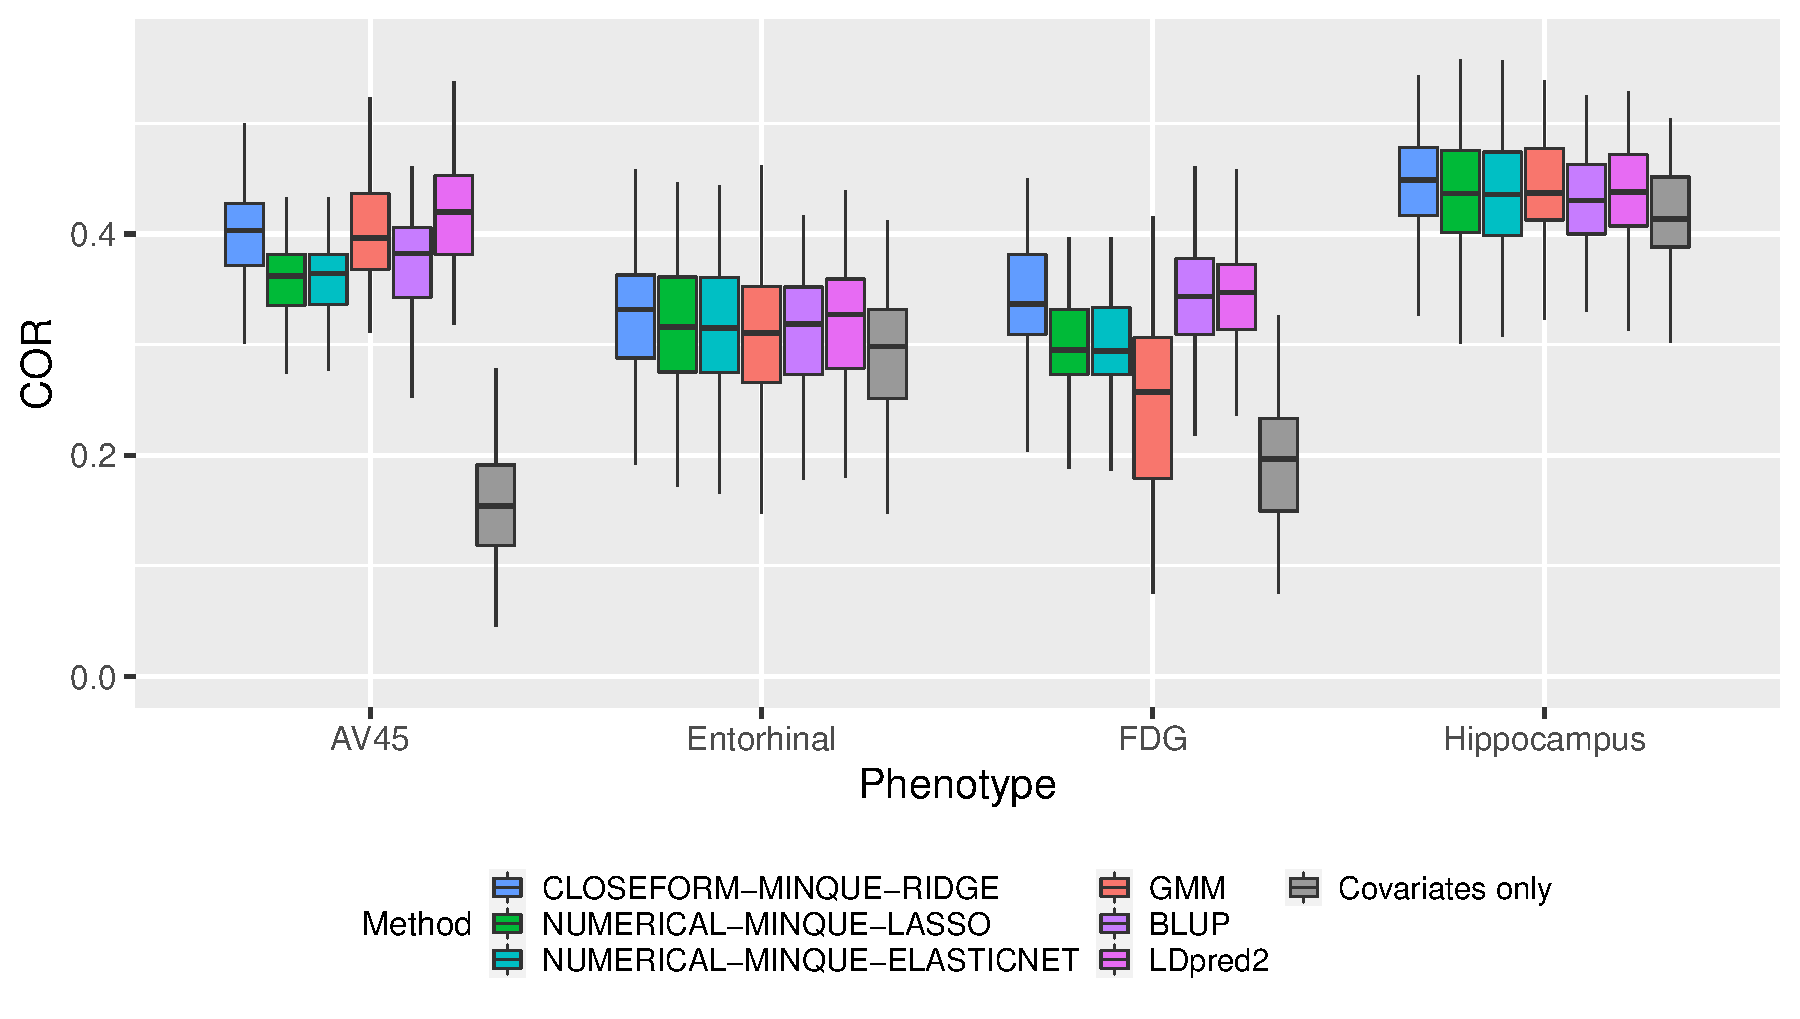
\includegraphics[width=\textwidth]{realdata_exp1.pdf}
  \caption{Prediction accuracy on ADNI using eleven candidate genes, one kernel
  per gene.  Each box summarises the correlation between predicted and observed
  phenotype in the held-out set over 100 random training/testing splits, with
  all methods evaluated on identical splits within each replicate.  The four
  phenotypes are amyloid burden (AV45), entorhinal cortical thickness, cerebral
  glucose metabolism (FDG) and hippocampal volume.  The covariates-only model
  gives the reference level attributable to age, sex and education alone.  For
  the proposed estimator the ridge penalty is chosen by five-fold
  cross-validation inside each training set, and the kernels are left
  unnormalised; no post-hoc adjustment is applied to any method.}
  \label{fig:adni-exp1}
\end{figure}


% --------------------------------------------------------------- Figure 15
\begin{figure}[htbp]
  \centering
  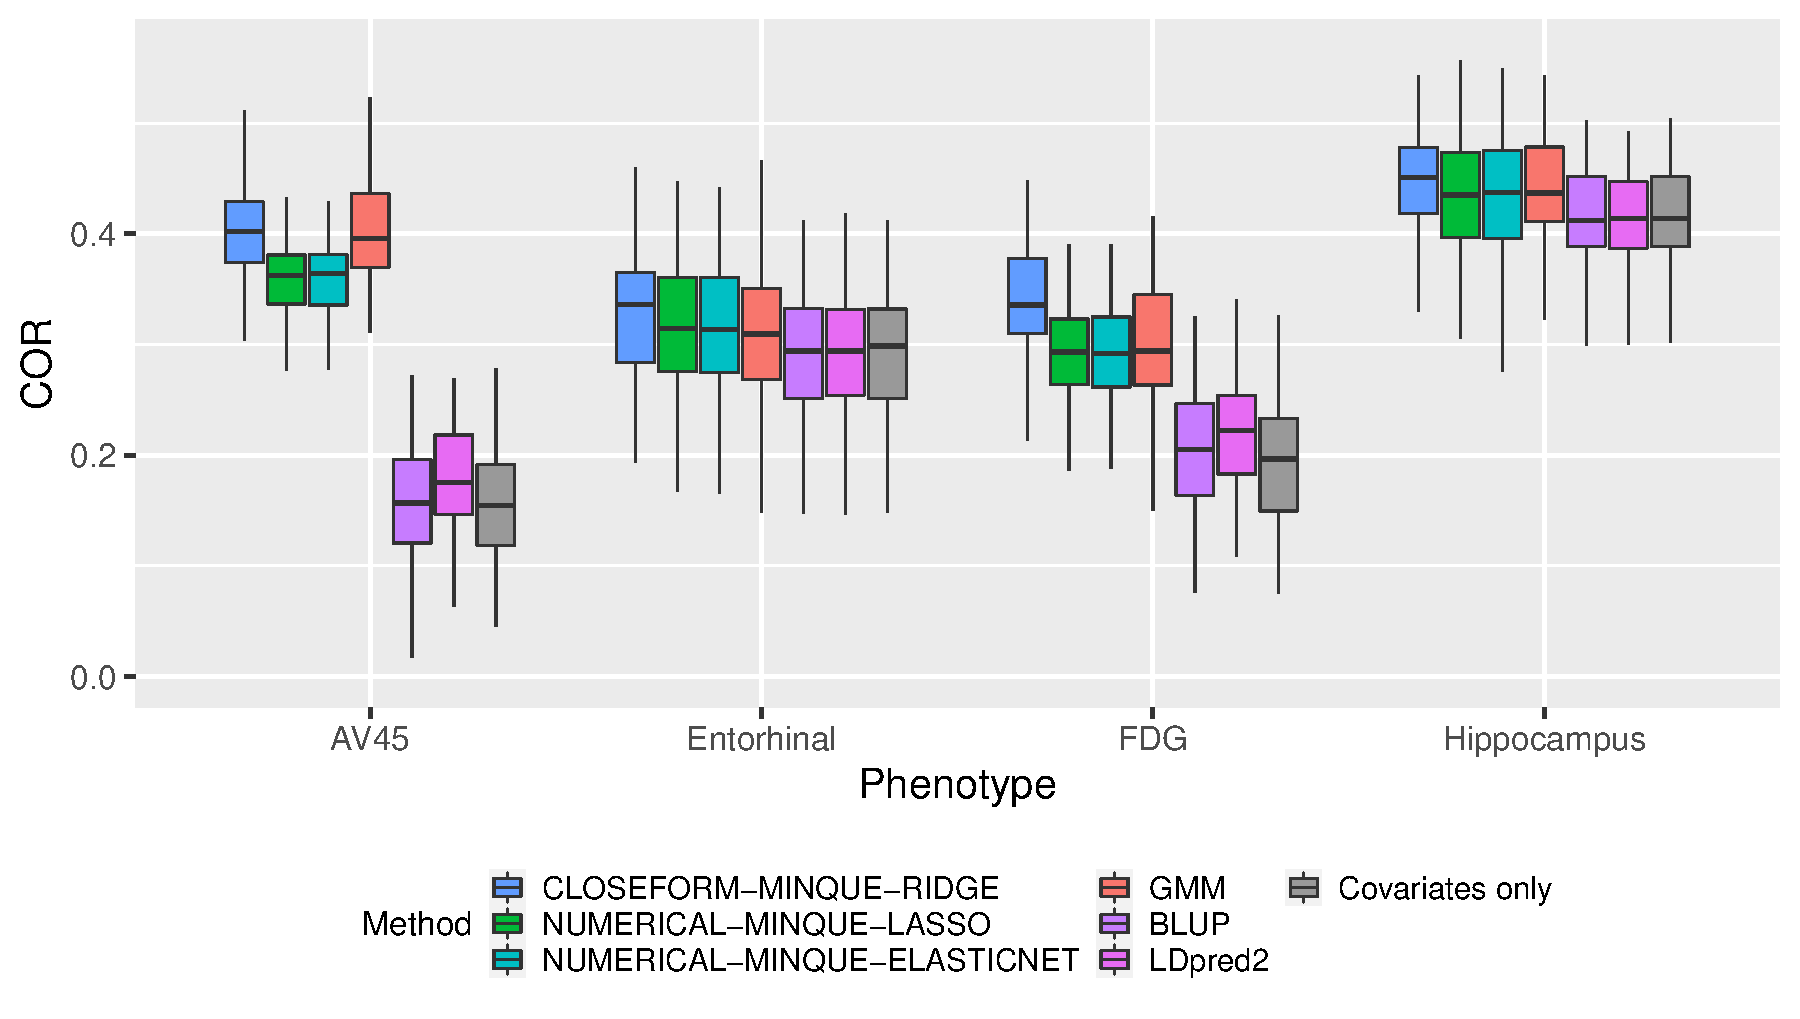
\includegraphics[width=\textwidth]{realdata_exp2.pdf}
  \caption{Prediction accuracy on ADNI when the rest of the genome is added as a
  twelfth kernel.  The eleven candidate gene kernels are retained and a single
  additional kernel is accumulated over all remaining genes as
  $\sum_g X_g X_g^{\top} / M$, so that variance not attributable to the
  candidate set can be absorbed rather than forced into the candidate
  components.  Phenotypes, splits, replication and tuning follow
  Figure~\ref{fig:adni-exp1}, and the splits are the same ones, so the two
  figures are directly comparable.  The comparison addresses whether the
  candidate gene restriction is doing the work, or merely discarding signal.}
  \label{fig:adni-exp2}
\end{figure}


% --------------------------------------------------------------- Figure 16
\begin{figure}[htbp]
  \centering
  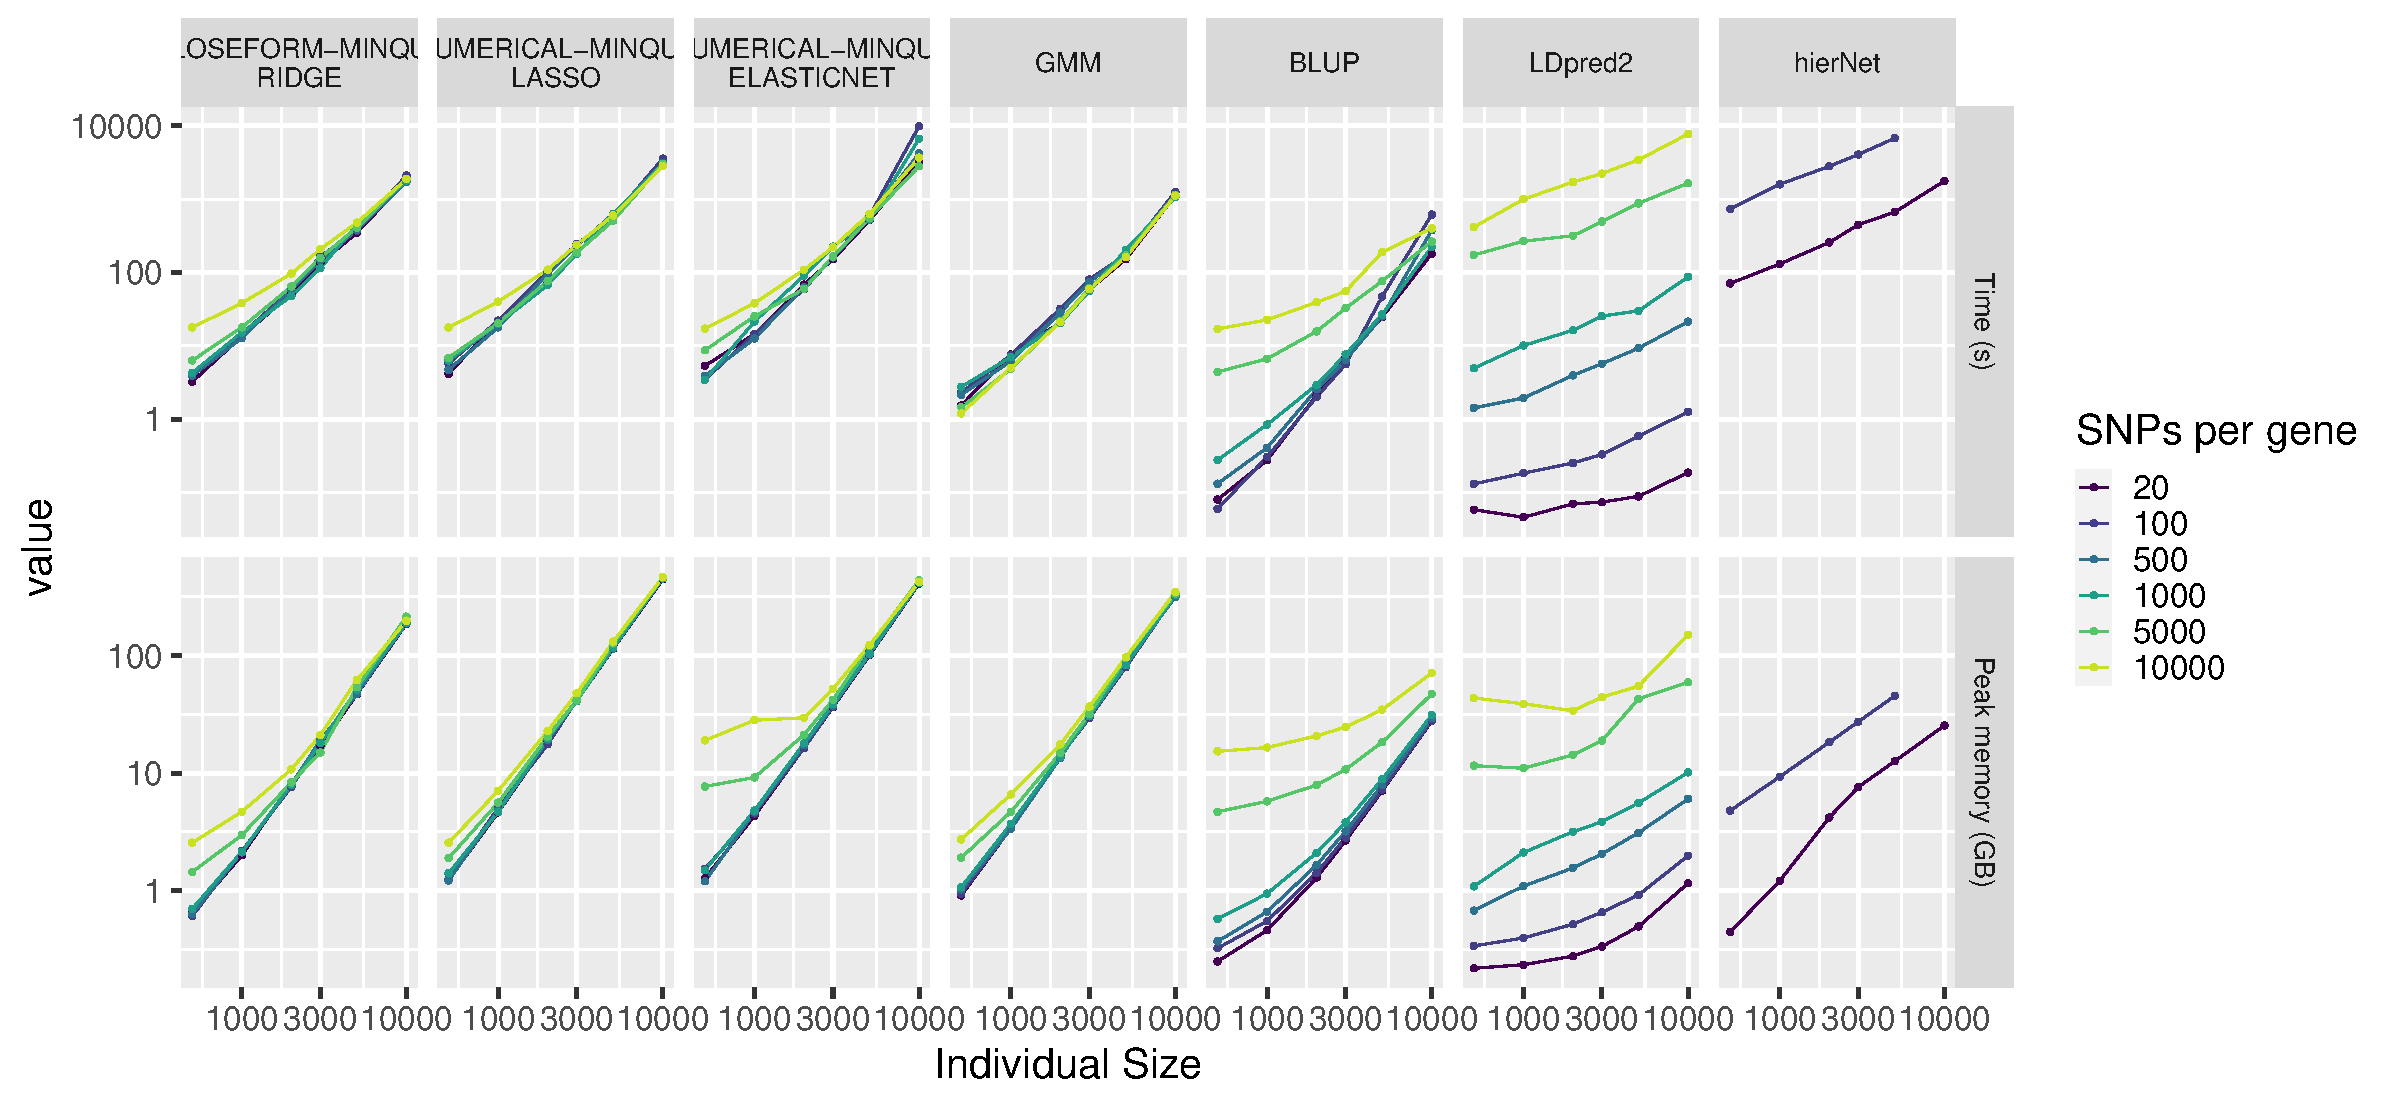
\includegraphics[width=\textwidth]{runtime_memory.pdf}
  \caption{Computational cost as a function of sample size and SNP density.
  The upper row reports wall-clock time in seconds and the lower row peak
  resident memory in gigabytes, one column per method, all on the interaction
  basis with ten regions and 67 components.  Sample size runs from 500 to
  10\,000 and SNP density from 20 to 10\,000 per gene; both axes are on a
  logarithmic scale, as the values span roughly five orders of magnitude.
  Unlike every other figure in this article, colour encodes SNP density rather
  than method, method being given by the column.  The two cost profiles are
  opposite: the kernel-based methods are essentially flat in SNP count and grow
  with sample size, because they operate in an $n \times n$ space, whereas
  LDpred2 is the reverse, growing from 0.2 to 7\,700 seconds as density
  increases at $n=10\,000$, because it operates per SNP.  hierNet stops after
  100 SNPs per gene, where the number of pairwise terms exceeds the 32-bit
  indexing limit of its compiled back end.  BLUP and LDpred2 are cheaper partly
  because they fit smaller models, an additive genomic relationship matrix and a
  linear polygenic score respectively; the like-for-like comparison on the same
  67-component basis is the closed-form ridge estimator against the two
  numerical MINQUE variants.}
  \label{fig:runtime-memory}
\end{figure}
